\documentclass[12pt]{report} % article, letter, book, macthesis, report, memoir, elsarticle

%Packages
\usepackage{graphicx} % This allows to include figures (images).
\usepackage{fullpage} % For using more space in paper (smaller margins).
\usepackage{pdfpages} % For including PDF Pages
\usepackage{todonotes} % For using notes
\usepackage{subfigure} % Allows to nicely group figures.
\usepackage[numbib,notlof,notlot,nottoc]{tocbibind} % Show "References" section in ToC.
\usepackage[hidelinks]{hyperref} % For hyperlinks.
\usepackage{footnoterange} % Allows to add footnotes.
\usepackage[T1]{fontenc}
\usepackage{titlesec, blindtext, color}
\usepackage{siunitx}
\usepackage{tabulary}
\usepackage{listings}

\graphicspath{{images/}}

\setcounter{secnumdepth}{3} % Depth of section numbering (will show numbers for subsubsections).
\setcounter{tocdepth}{3} % Depth of subsection showing in ToC.

% Spacing between paragraphs.
\setlength{\parindent}{0in} 
\setlength{\parskip}{3mm}

% References
\renewcommand{\bibname}{References} % Change "Bibliography" name to "References"

% Chapter titles
\definecolor{gray75}{gray}{0.75}
\newcommand{\hsp}{\hspace{20pt}}
\titleformat{\chapter}[hang]{\Huge\bfseries}{\thechapter\hsp\textcolor{gray75}{|}\hsp}{0pt}{\Huge\bfseries}

%PDFPage Counter for Appendix files
\newcounter{includepdfpage}


\usepackage{xcolor}

\colorlet{punct}{red!60!black}
\definecolor{background}{HTML}{EEEEEE}
\definecolor{delim}{RGB}{20,105,176}
\colorlet{numb}{magenta!60!black}

\lstdefinelanguage{json}{
    basicstyle=\normalfont\ttfamily,
    numbers=left,
    numberstyle=\scriptsize,
    stepnumber=0,
    numbersep=8pt,
    showstringspaces=false,
    breaklines=true,
    frame=lines,
    backgroundcolor=\color{background},
    literate=
     *{0}{{{\color{numb}0}}}{1}
      {1}{{{\color{numb}1}}}{1}
      {2}{{{\color{numb}2}}}{1}
      {3}{{{\color{numb}3}}}{1}
      {4}{{{\color{numb}4}}}{1}
      {5}{{{\color{numb}5}}}{1}
      {6}{{{\color{numb}6}}}{1}
      {7}{{{\color{numb}7}}}{1}
      {8}{{{\color{numb}8}}}{1}
      {9}{{{\color{numb}9}}}{1}
      {:}{{{\color{punct}{:}}}}{1}
      {,}{{{\color{punct}{,}}}}{1}
      {\{}{{{\color{delim}{\{}}}}{1}
      {\}}{{{\color{delim}{\}}}}}{1}
      {[}{{{\color{delim}{[}}}}{1}
      {]}{{{\color{delim}{]}}}}{1},
}

% CONTENT
\begin{document}

\begin{titlepage}
	\begin{center}
		\vspace*{1cm}
		
		\Huge
		\textbf{Occupancy Analyzer}
		
		\vspace{0.5cm}
		\LARGE
		Detection and prediction of occupancies with limited ressources
		
		\vspace{1.5cm}
		
		\textbf{
			Christoffer Wilken Pagaard\\
			Jacob Romme Rasmussen\\
			Theresa Brandt von Fackh\\
			Tomas Miseikis\\
		}
		
		\vfill
		
		Report
		
		\vspace{0.8cm}
		
		
\includegraphics[width=0.4\textwidth]{ITU_logo_ENG}
		
		\Large
		Denmark\\
		15. December 2013
		
	\end{center}
\end{titlepage}

\newpage % Makes a new page.

\newpage

\tableofcontents

\newpage

\chapter{Introduction}
\label{introduction}
\section{Context}
\label{sec:Context}

%given whatever a 1st semester MSc student from ITU knows
%What the audience needs to know in order to start reading this report.
%To bring the reader up to a level that allows you to tell your story.
%Course setup
%Aim for 1 page.

Smart use of energy resources is an ongoing topic these days. The reduction of expenses is mostly the biggest driving factor for companies. But also the debate around climate change brings new legislation to reduce the waste of energy resources, whose production is damaging to the environment and future generations. The IT University of Copenhagen (ITU) has an interest in producing an occupancy model for commercial buildings, like the ITU building, to detect where energy resources are needed and where they can be saved. Energy resources are needed for e.g. lighting and heat-regulating systems, which are relevant for occupants in a commercial building. With the detected occupancy data the ITU can predict occupancy and develop concepts for a smart use of energy resources in commercial buildings.

The Strathmore University in Kenya has also an interest in building up an occupancy model, but mainly for surveillance reasons. Surveillance can be used for several purposes like traffic monitoring, public safety and facilities surveillance. An IT-based surveillance system can automatically analyze the scene without the use of human resources. By analyzing the scene the detection of occupancy is a major part. Moreover a real-time prediction model on top of the occupancy data can be used to prevent criminal activity by triggering alarms or other surveillance systems.

Currently there is no existing infrastructure to build up an occupancy model in the Strathmore University or the ITU building. Both universities want a solution for an occupancy analyzer based on Raspberry Pi computers due to the minimal consumption of computational and monetary resources. Furthermore, Starthmore University requests for an Android application, which represents a live-feed of the occupants in a monitored room.

A group of students from both universities have to collaborate to come up with a solution for an occupancy analyzer, which can satisfy the needs of both university interests. Ideally a product should be developed, which can be adapted to fit the needs of one or the other university.
Furthermore, a collaboration project is mandatory for the student group from ITU, in which they have to face the challenges of global collaboration, navigate compromises and come up with a solution.

This report contains the product result, design of the product, details of the project work and the learning outcomes, which were achieved in the project with the globally distributed team from the perspective of the ITU students. The project team consists of international students located in Nairobi, Kenya (East African Time) and Copenhagen, Denmark (Central European Time).


\section{Problem}
\label{sub:problem}
%given the context
%What is the specific problem you are looking at? At this point this won't be clear to you and that is okay. Spend some time thinking about what the system you are building could be used for and write down something that makes sense (notice that this is the reverse approach: what do we want to do -> what does this solve).This makes you think about the problem and gives us something to discuss. Later on we will revise it. 
%Describe the problem you are facing.
%Give a clear definition of the problem you are trying to solve. This is what the success of the product is measured against.
%The context
%Aim for ½-1 page.

The content of this project is to build an occupancy analyzer, which detects people in a room or corridor and predicts their movement. The occupancy analyzer has to be based on Raspberry Pi computers, which come with computational restrictions, and web cameras. A solution for the right architecture and programming languages has to be found, which can deal with those limited resources.

Due to the usage of web cameras, a visual detection of people has to be made. Analyzing images by detecting people - which are moving objects and not part of the room - is one major challenge to face. Visual conditions of the image can change as a result of daylight. For example, dynamic lighting and moving shadows should not influence the detection of people. 
To best capture occupants and the requirement to represent the occupants on an Android application, the position of web cameras becomes an important factor.
The differentiation between multiple people, as well as between people and the setting of the room, is important for the quality of the detection. Only if reliable data about occupancy exists, can the data be used to construct a reliable prediction model usable for future concepts and projects.

The question of how the collected data can be used, has to be considered. Building prediction models, which relies on historical data and real-time data, is another requirement, which the project dealt with. Decisions on what kind of prediction for a meaningful application - like the one mentioned in paragraph 2 in Section~\ref{sec:Context} - and how the data will be stored and processed have to be made.

Besides the design and implementation of an occupancy analyzer, another task is the collaboration of students from two different universities. Cultural differences, difference in time, spatial distance and locally related influences have to be overcome. Different perspectives have to be combined and compromises have to be made.

\section{Related Work}
\label{sub:related}
%given the poblem
%What have other people done that is relevant to your problem and what can we learn from them. Start by writing a list of paragraphs. Each should describe one related work, where it did well in respect to your specific problem and where it falls short of solving this. 
%Looking back, what have others done that is relevant to the problem?
%To show that you have done your homework and surveyed existing solutions.
%The problem
%The Internet; in particular: ACM http://dl.acm.org; IEEE http://ieeexplore.ieee.org
%What is the core of each contribution?
%How does this apply to your specific problem?
%What can you build on and what is missing?
%Aim for 1-2 pages.

%NREL IPOS Project:
%http://techportal.eere.energy.gov/technology.do/techID=986
%http://www.nrel.gov/news/features/feature_detail.cfm/feature_id=2210
%http://e3tnw.org/Documents/IPOS%20Presentation.pdf
%http://www.ibpsa.us/presentations/2013.06_IBO_Boulder/Thursday/Low-Cost%20Sensing/Low-Cost%20Sensing_L_GENTILE_POLESE.pdf
%http://m.eetasia.com/ART_8800686058_480500_NT_509225b4.HTM


%http://ieeexplore.ieee.org/xpl/login.jsp?reload=true&tp=&arnumber=5606357&url=http%3A%2F%2Fieeexplore.ieee.org%2Fiel5%2F30%2F5606236%2F05606357.pdf%3Farnumber%3D5606357

%The concept of an occupancy analyzer, which uses visual recognition of occupants, is already handled in several papers and projects. \\
%Some guy investigated something about some image analysis and or occupancy analysis. \\

Background subtraction is an extremely important concept in surveillance applications, since this is the first step in detecting people and tracking their movement in monitored area. Y. Benezeth, P.-M. Jodoin, B. Emile, H. Laurent \& C. Rosenberger~\cite{simple_background_subtraction}, in their work \emph{Comparative Study of Background Subtraction Algorithms}, mention a basic motion detection approach by using a simple background subtraction technique. In this technique, the background image is taken when there is a total absence of motion in the monitored area. This background image is then subtracted from every newly taken image of the area in order to detect motion. This is possible since after subtraction the resulting image will either be almost totally black - meaning no motion occurred - or the image will have some resulting bright contours of detected differences.

We intend to apply this simple technique in the beginning of the project for the initial experiments and studies of object detection and tracking. We expect that these experiments and studies will provide us with some knowledge on how basic object detection works and how we can apply it for our specific problem.

Aditi Jog \& Shirish Halbe~\cite{jog_halbe}, in their paper \emph{Multiple Object Tracking using CAMshift Algorithm in Open CV}, present a better way of building object detection and tracking application than simply using the basic background subtraction approach. For their implementation they build upon an existing algorithm called CAMshift~\footnote{Continuously Adaptive Mean Shift.}, which is capable of tracking multiple moving objects in video streams. In this algorithm, an approximate background image of the monitored area is gradually built up by smoothing or blurring out the motion areas. This is done by using several recent images of the monitored area, and performing arithmetic averaging on them. One can then simply use this built up background image for detecting changes in the monitored area.

This approach applies to the first part of our problem, namely detecting and tracking people in the monitored area. We can build upon this approach as the implementation of it is quite simple yet flexible and adaptive. Moreover, it eliminates the need to worry about fluctuations in lighting and other unpredictable changes in the background that may corrupt the interpretation of the monitored area.

Gellert \& Vintan~\cite{gellert}, in their work \emph{Person Movement Prediction Using Hidden Markov Models}, presents the use of hidden Markov models to anticipate the next movement of a given person. It is used inside an office building where it is possible to predict which room a person will enter next based on the history of rooms visited. The configuration of the model is optimised by evaluating movement sequences of real persons within an office building.

The idea of predicting which room a person will enter next can be used in our scenario to predict which area of the room a person will occupy next. This information can be used in the process of predicting where a person will exit the room.

Ashbrook \& Starner~\cite{ashbrook} demonstrated how locations of significance can be incorporated into a predictive model in the paper \emph{Using GPS to Learn Significant Locations and Predict Movement Across Multiple Users}. They cluster location data from a GPS over an extended period of time and infer meaningful locations. These locations are then incorporated into Markov models where it is used to predict a person's future location given any current location. The idea of using heavily visited areas, that is \emph{locations of significance}, to perform predictions can be transferred to our scenario, where each area of the image can be mapped to a value reflecting the amount of activity within the area. This value plays an important role in the calculations of probabilities and thereby the final predictions.

\section{Approach}

%given the problem and the related work
%How do you intend to solve the problem? 
%To give a summary of how you did things.
%How do you propose to solve the problem? Or at least, how do you propose to take a step towards a solution for the problem?
%Aim for 1 page.
Given the problems listed in section \ref{sub:problem} and the related work listed in section \ref{sub:related}, we propose a system consisting of three webcams, three Raspberry Pis, a single server and an android application. Each webcam is placed in a seperate room recording occupant activity. The webcam is connected to a Raspberry Pi performing analysis on the images received from the cameras. The analysis is made to detect occupants within the image and the information is sent and stored on the server. The android application can request information about the locations of each occupant and predictions about a single occupant. A prediction is essentially a guess about where an occupant will exit a room based on historical data. At any point during the presence of an occupant a prediction can be requested. \\
Due to the limited computation capabilities of the Raspberry Pis we have to perform benchmarks to find the appropriate programming language and framework for image analysis. For occupant detection, we gradually build up an approximate background image of the monitored area by smoothing and blurring out the areas with activity. The background image is compared to a given image where the difference displays where exactly activity has taken place. \\
We choose to follow a client-server approach where all communication from and to the devices and database goes through the server. The prediction logic is stored on the server as well and will be based on the approach laid out by Gellert \& Vintan\cite{gellert}. Instead of transitions between office rooms we split the image into sections and calculate probabilities of transitioning to other image sections. Our prediction approach is derived from the hidden Markov Models where we use historical data the past amount of activity in each image section in the calculations. \\
The design and implementation of the android application is assigned to the Kenyan team with whom we will come to mutual agreements about the data sent from the server and what prediction information can be requested. These decisions will be agreed upon during weekly meetings and regular email correspondences.

\section{Report Structure}
%This is one easy paragraph that you write the last week.
%How is the report structured?
%Give a quick hint of the layout of the report
%For each top-level section write a sentence describing the section. Make sure those sentences are linked.
Section \ref{analysis} analyses the problems presented in section \ref{sub:problem} and presents and discusses various solutions. Based on the discussions, section \ref{design} presents the final system design. Any implementation specific details about the system that are deemed not immediately obvious will be covered in section \ref{implementation}. Section \ref{evaluation} evaluates the results from tests of the final system. The whole project process including management, issues and collaboration with the Kenyans is covered in section \ref{collaboration}. Finally, the system and project process will be concluded in section \ref{conclusion}.

\chapter{Analysis}
\label{analysis}
\section{Image Analysis}
\label{sec:analysis_img}
There are numerous factors that must be considered when designing a surveillance system.

{\bfseries Position of the camera.} Camera's type, position and angle may differ a lot, depending on the requirements of the surveillance application. In our scenario it was determined that the most optimal position of the camera would be the ceiling, making the camera point down to the monitored area. This would provide us with an increased field of view, and would make detection of multiple people walking side by side easier. However, due to resource limitations and difficulties we would face trying to position the camera in such way, decision was made to simply place the camera on a higher floor and point it down to the monitored area in approximately 50-60\si{\degree} angle.

{\bfseries Object Extraction.} As we have already touched a bit in Related Work section, background subtraction plays an important role in detecting people and tracking their movement. There are multiple ways in dealing with background subtraction, but we have mainly covered two - simple background subtraction - where we use a static background image to detect difference in frames - and running average approach - where we gradually create an approximate background image to extract moving objects from the frame. The former approach can work rather poorly and inaccurately in dynamic environments, whereas the latter one deals with the same challenges in a better way, thus have been chosen for our design. This is further discussed in greater detail in Section~\ref{sec:object_extraction}.

{\bfseries Object Detection.} To build up a complete and reliable surveillance system, one must be able to identify whether the detected object is a person, an animal or simply tree leaves moving because of wind. To deal with this, one can possibly apply face detection methods or object's shape recognition techniques. Since these are rather complicating areas in image processing, and our test scenarios mainly dealt with environments where the background is more stable, we did not consider object identification and simply interpreted all changes in the monitored area as human movement. Our object detection approach is explained in more detail in Section~\ref{object_detection}.

{\bfseries Object Differentiation.} Another important part of surveillance is being able to differentiation between multiple people crossing the monitored area. To deal with this challenge, we looked into two approaches, namely histogram approach - where we calculate individual histogram for every person and try to match it next time we detect people in the frame - and last coordinate approach - where we, instead of calculating person's histogram, calculate person's last coordinates in the monitored area. The main problem these both approaches share is that they are not very precise, however, the latter approach was easier to implement, thus was chosen for our design. Further comparison and discussion on object differentiation is provided in Section~\ref{object_differentiation}.

\section{Prediction}
\label{sec:analysis_pred}
In our scenario where occupants enter and exit the room constantly, typically within seconds or minutes of each other, it is somewhat difficult to find the immediate use of predicting an occupant's future actions. However, our partner team from Kenya expressed a need for such a system because they have had issues with thefts. Incorporating such a feature to their surveillance systems could warn a guard whenever suspicious activity might occur. A suspicious activity could involve a person moving too close to a given exit - possibly leading to a restricted area. In order to calculate a somewhat reliable prediction, we need to capture and store data about the behavior of previous occupants. When the data set grows, the prediction gradually becomes smarter and generally more precise. In order to satisfy the prediction requirement, various existing solutions have been considered, namely the \emph{k-nearest neighbors algorithm} and an existing prediction model, the hidden Markov model. The two solutions will be covered briefly. The former assigns a given object to a group depending on the \emph{k} nearest objects. To apply this to our scenario we imagined previously observed occupant positions being separated into groups dependent upon the chosen exit. Given any position we would analyze the \emph{k} neighboring previous positions of distinct occupants and predict the exit to be that of the majority.
\begin{figure}
\centering
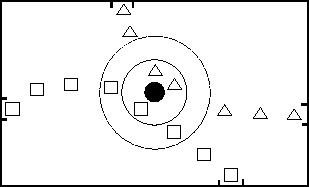
\includegraphics{prediction_figures/knn_room}
\caption{An illustration of the \emph{k-nearest neighbors algorithm}.}
\label{fig:knn}
\end{figure}
Figure~\ref{fig:knn} depicts an example where the center dot is the current position and the squares and triangles are previous occupant positions who chose separate exits. The circle with the solid line resembles a situation where \emph{k=3} which indicates that the occupant at the center is most likely to take the same exit as the occupants previously positioned at the triangle positions. The circle with the dashed line resembles a situation where \emph{k=5}. This yields a different output where the occupant is most likely to choose the same exit as the occupants previously residing at the positions of the squares. The approach has proven to be inefficient on larger data sets~\cite{bhatia}, which can be averted by performing clever data reduction. This, however, deemed the approach out of the scope of this project.
\begin{figure}
\centering
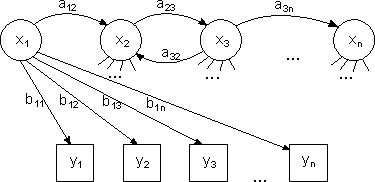
\includegraphics{prediction_figures/markov}
\caption{An illustration of the hidden Markov model.}
\label{fig:markov}
\end{figure}

Figure \ref{fig:markov} depicts the different parameters a hidden Markov model works with. Each \(x\) is a state and each \(y\) is a possible observation, where \(a\) is a state transition probability and \(b\) is an output probability. When translating this to our scenario we need to define what exactly a state and an observation is and how to calculate the different probabilities. Since the ultimate goal is to predict what exit an occupant is going to take, a possible observation could be that an occupant exits a room at a given location. A state could depict a room area where a transition to another room area would have a state transition probability \(a\). Given an occupant resides in any room area, \(b\) is the probability that the person will exit at a given location. Typically, the process is as follows; random probability values are assigned to \(a\) and \(b\) (maybe a ref to jahmm or something else). Gradually, these values are updated to reflect actual observed actions of occupants. Over time, the probabilities are modified and represent how the average occupant is moving given a current location, resulting in more accurate predictions - this process is commonly referred to as training. Even with the inclusion of a training procedure, the predictions will be incredibly unreliable in the beginning until a large enough data set has been collected. (DISCUSS, this might be wrong) Furthermore, imagine a scenario where an even number of occupants move from one exit to another in both directions, evenly split. At any location along the path the probabilities to each exit remain equal, since equally many previous occupants have taken each exit given the current location. In an attempt to partially avoid these issues, or at least produce some more reliable results with lesser data sets, we wanted to establish rule sets and integrate those into the calculations. Thus, we chose to design our own prediction model, heavily inspired by the hidden Markov model, since the original interpretation of states and probabilities as depicted in figure \ref{fig:markov} is maintained. The custom model is explained in detail in Section~\ref{ssub:designcustomprediction}. 

\chapter{Design}
\label{design}
\section{System Overview}
Figure~\ref{fig:system_overview} displays the different components in the system and how they relate and communicate with each other.
% Tomas' system overview.
\begin{figure}[ht]
	\centering
	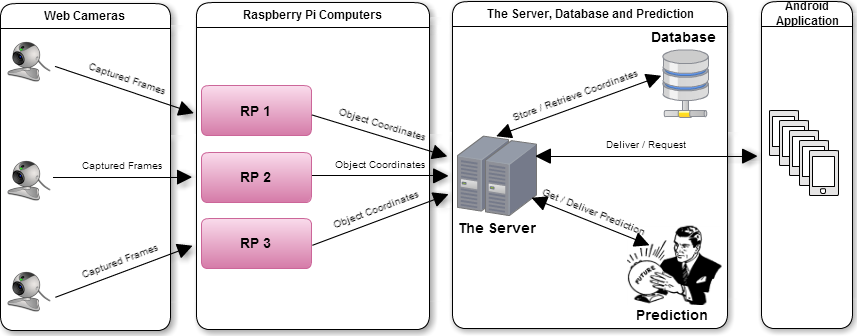
\includegraphics[scale=0.89]{system_overview/system_overview_tomas}
	\caption{Occupancy Analyzer System Overview}
	\label{fig:system_overview}
\end{figure}

As we can see, the system primarily consists of 4 components:

\begin{enumerate}
	\item Web cameras,
	\item Raspberry Pi computers,
	\item The server,
	\item and the Android application.
\end{enumerate}

All of these components are discussed further on in the respective chapters.

%camera placement and positioning reference: http://www.lorextechnology.com/support/self-serve/Camera-Location-Placement-and-Positioning/2700036
\section{Web Cameras}
The purpose of the web cameras is simply to surveillance the area they have been placed in and forward the captured frames to Raspberry Pi computers for further processing, as shown in Figure~\ref{fig:system_overview}. The cameras can be placed in a room, corridor, atrium or any other similar place in or outside of the building, where the services offered are required. Cameras can be placed either directly above the observed area (Figure~\ref{fig:camera_top}) or in the corner of it, as illustrated in Figure~\ref{fig:camera_corner}. Naturally, a camera placed above the observed area would give better results, since this increases its field of view and makes it easier to correctly detect and distinguish between multiple people walking side by side. Furthermore, for the best results one must also take many different factors into account, such as
the distance between the camera and monitored area, environmental conditions of the area the camera is placed in, lighting conditions.

% Camera top placement.
\begin{figure}[ht]
	\centering
	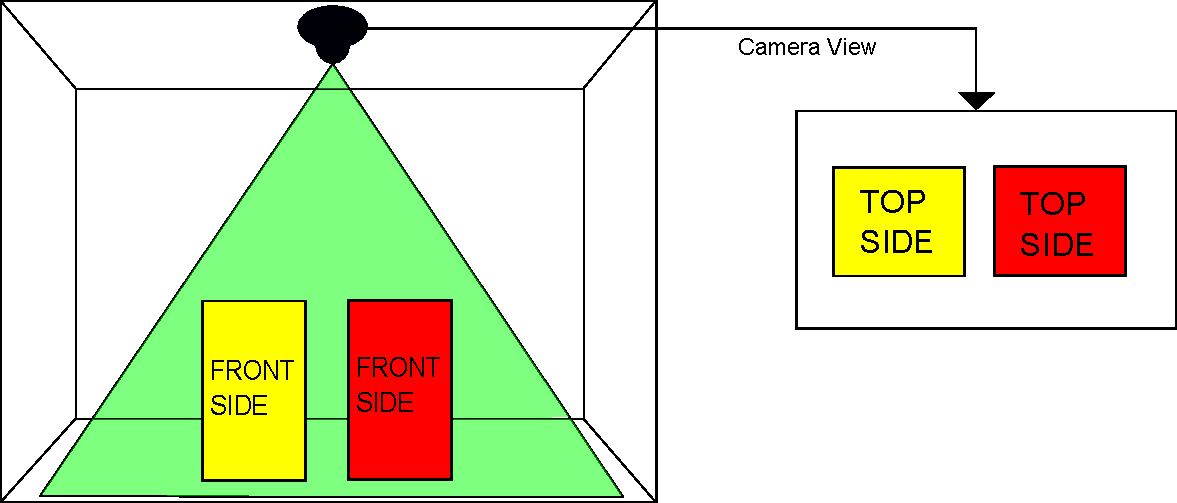
\includegraphics[scale=0.82]{camera_placement/camera_top}
	\caption{Camera top placement}
	\label{fig:camera_top}
\end{figure}

% Camera corner placement.
\begin{figure}[ht]
	\centering
	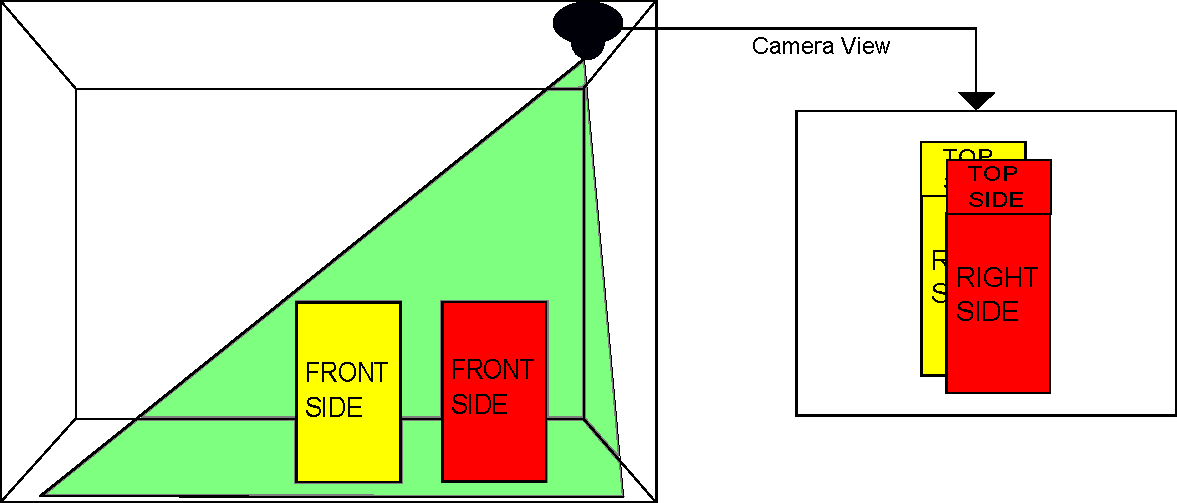
\includegraphics[scale=0.82]{camera_placement/camera_corner}
	\caption{Camera corner placement}
	\label{fig:camera_corner}
\end{figure}

\section{Raspberry Pi Computers}
The next component in the system architecture is Raspberry Pi computers. These computers have at least one web camera attached to them, and are responsible for processing the frames captured by these cameras. The main goal of processing these frames is to try to detect people in the monitored area and determine their position in that area. There are many different challenges in object detection, as well as various concepts and techniques that can be used to achieve this. We discuss these in the next sections.
	
	\subsection{Object Extraction}
	To detect and extract objects, or in our case, people and their movement, we need to apply several motion detection techniques on the frames we are receiving from the web camera. First of all, to detect changes in some monitored area, we naturally need to have at minimum two images, which we must compare to see what changes occurred. We will try to look into two different approaches in doing this, a simple one, and one that is a bit more complicated and sophisticated, but much more adaptive and flexible.
	
	\subsubsection{Background Subtraction Approach}
	A simple approach - called Background Subtraction - would be to have a static background image of observed area that was taken prior to the analysis and did not have any people in it. Then, one can simply detect changes and movement in the area by subtracting the static background image from every newly taken image of the monitored area~\cite{background_subtraction_1}. The difference between the two images would then allow us to see if any changes happened, since after subtraction the resulting image would either be almost totally black (Figure~\ref{fig:background_subtraction_1}) - meaning no one walked passed the observed area - or the image would have some resulting bright contours of detected differences (Figure~\ref{fig:background_subtraction_2}).
	% Background Subtraction with no background changes.
	\begin{figure}[ht]
		\centering
		
\includegraphics[scale=0.82]{background_subtraction/background_subtraction_1}
		\caption{Background Subtraction with no background changes}
		\label{fig:background_subtraction_1}
	\end{figure}
	% Background subtraction with background changes (lego man appearing).
	\begin{figure}[ht]
		\centering
		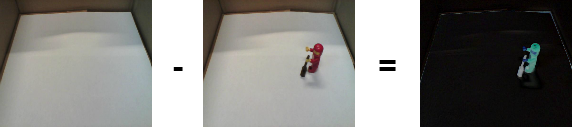
\includegraphics[scale=0.81]{background_subtraction/background_subtraction_2}
		\caption{Background Subtraction with background change}
		\label{fig:background_subtraction_2}
	\end{figure}
	
	After doing some research and experimenting with background subtraction technique, one will quickly discover that there are multiple weaknesses to it. 
	
	\begin{itemize}	
	\item First of all, if the initial background image is always static and never changes, this technique will fail in environments where lighting is dynamic. This is perfectly illustrated in Figure~\ref{fig:background_subtraction_3}. We can see that the lighting is much darker in the second image, possibly because the light was turned off in the monitored room, thus after subtracting our static background image from this image, the resulting image is simply a lighter version of the two images, and not the intended black image. The reason why this happens is because the original brighter background image has a much higher intensity, thus the average value of it's pixels are higher than the pixel values of the newly taken darker image. Naturally, this is a big problem, because now even if a person moves through the monitored area (Figure~\ref{fig:background_subtraction_4}), he or she will not be as easily extractable as in Figure~\ref{fig:background_subtraction_2}.
	% Background subtraction with background changes (lighting changes).
	\begin{figure}[ht]
		\centering
		
\includegraphics[scale=0.82]{background_subtraction/background_subtraction_3}
		\caption{Background Subtraction with background lighting change}
		\label{fig:background_subtraction_3}
	\end{figure}
	% Background subtraction with background changes (lighting changes + lego figure).
	\begin{figure}[ht]
		\centering
		
\includegraphics[scale=0.81]{background_subtraction/background_subtraction_4}
		\caption{Background Subtraction with background lighting change and lego figure appearing}
		\label{fig:background_subtraction_4}
	\end{figure}
	
	\item Another problem with background subtraction approach surfaces when a camera is placed inside an area which has objects that constantly change their original position (chairs, tables, appliances, etc.) by being moved, even small changes in object's location will spoil the resulting image after subtraction. As we can see in Figure~\ref{fig:background_subtraction_5}, the object is displayed twice in the resulting image, even thought we were not even interested in it, making it much harder to detect actual people moving in the area. From now on, the resulting image after subtraction will always be corrupt unless the object is placed back in its original position.
		% Background subtraction with background changes (object changes location).
	\begin{figure}[ht]
		\centering
		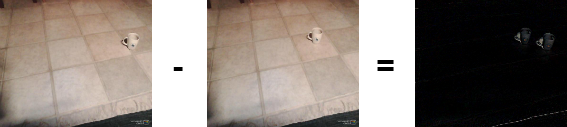
\includegraphics[scale=0.82]{background_subtraction/background_subtraction_5}
		\caption{Background Subtraction with object changing it's location}
		\label{fig:background_subtraction_5}
	\end{figure}
	\end{itemize}
	
	In conclusion, we can see that simple background subtraction approach can work well in static environments, however it falls short in dynamic spaces. Naturally, these mentioned drawbacks of background subtraction approach need to be handled for object detection to work well, which creates additional challenges when implementing the system.

	\subsubsection{Running Average Approach}
	\label{sec:running_average_approach}
	A much better approach for movement detection is using a running average method. In this technique we do not need to rely on a static background image of the monitored area taken prior to analysis. Instead, we try to find a new "approximate" background image by interpreting any changes in the background as noise and blurring them out. This is accomplished by taking a train sequence of multiple previously captured frames and performing arithmetic averaging on that sequence~\cite{running_average_approach_1}. This exact approach is illustrated in Figure~\ref{fig:running_average_example}. As we can see, hand motion moving up and down (Figures~\ref{fig:running_average_1},~\ref{fig:running_average_2} and~\ref{fig:running_average_3}) gets blurred out when applying running average method, thus producing an approximate background image (Figure~\ref{fig:running_average_4}) that can be used for subtraction of the test frames from it. This method of object extraction works very well and has a lot of flexibility. It can adapt to environmental changes in the monitored area, thus eliminating most of the weaknesses that the background subtraction approach has. For these reasons, the running average approach was chosen for our design.
	% Running average example.
	% subfigure allows to group figures and put them next to each other.
	\begin{figure}[ht]
		\centering
		\subfigure[Test frame 1]{
		
\includegraphics[scale=0.40]{running_average/running_average_1}
		\label{fig:running_average_1}}
		\quad
		\subfigure[Test frame 2]{
		
\includegraphics[scale=0.40]{running_average/running_average_2}
		\label{fig:running_average_2}}
		\subfigure[Test frame 3]{
		
\includegraphics[scale=0.40]{running_average/running_average_3}
		\label{fig:running_average_3}}
		\quad
		\subfigure[Running Average frame]{
		
\includegraphics[scale=0.40]{running_average/running_average_4}
		\label{fig:running_average_4}}
		\caption{Example of Running Average technique}
		\label{fig:running_average_example}
	\end{figure}
	\subsection{Object Detection}
	Now that we can extract objects using running average technique, we need to be able to actually find them in the resulting image we get after we perform subtraction. For this, we need to apply several key techniques in image processing. 
	
	\begin{itemize}
	\item After we capture the initial frame of the monitored area, it will often contain noise and small details that we are not interested in. To deal with this, we must first apply blur or smoothing filter. In blurring technique we calculate weighted averages of areas of pixels in a source image by passing through it~\cite{blur_1}, which helps to reduce image noise and detail, as shown in Figure~\ref{fig:blur_example}.
	% Blur example.
	\begin{figure}[ht]
		\centering
		\subfigure[Original frame]{
		
\includegraphics[scale=0.40]{blur/blur_1}
		\label{fig:blur_1}}
		\quad
		\subfigure[Frame after blur is applied]{
		
\includegraphics[scale=0.40]{blur/blur_2}
		\label{fig:blur_2}}
		\caption{Blur example}
		\label{fig:blur_example}
	\end{figure}
	
	\item After we remove the initial noise, we can perform subtraction using running average approach (described in Section~\ref{sec:running_average_approach}). After subtraction we will either get a nearly totally black image, meaning no motion occurred, or an image where some colors stand out, meaning some motion has occurred. 
	
	\item In either case, for further processing of the taken frame, we can choose to convert it to a grayscale image. The reason for this is that the original RGB image we get has three channels, while grayscale image has only one~\cite{grayscale_1}, thus it is easier to work with. This procedure is illustrated in Figures~\ref{fig:grayscale_1},~\ref{fig:grayscale_2} and~\ref{fig:grayscale_3}. 
	
	\item For further processing of the image, we apply threshold technique, which converts the image to black and white and removes some more unwanted details and noise~\cite{threshold_1}. After threshold is applied we get the image shown in Figure~\ref{fig:threshold_1}. 
	
	\item Moreover we want to expand the interesting parts of the image and contract smaller pieces, which can be considered noise and managed to slip through, even after we performed thresholding. To do so, we use two fundamental operations in morphological image processing, that is, dilation and erosion. Dilation allows us to expand the shapes contained in the image~\cite{dilation_1}, whereas erosion simply shrinks shapes~\cite{erosion_1}, so that bright regions surrounded by dark regions shrink in size, and dark regions surrounded by bright regions grow in size. When we apply dilation and erosion we get the image shown in Figure~\ref{fig:dilate_erode_1}. 
	
	\item Now, to project the detected area onto the original frame, we simply use bounding box technique, which gives us the coordinates of the rectangular border that fully covers the extracted white silhouette~\cite{bounding_box_1} that we got in~\ref{fig:dilate_erode_1}. Then we use these coordinates to draw a simple rectangle, as well as mark it's middle position by a red circle, as illustrated in Figure~\ref{fig:bounding_box_1}.
	\end{itemize}
	\begin{figure}[ht]
		\centering
		\subfigure[Original frame]{
		
\includegraphics[scale=0.65]{grayscale/grayscale_1}
		\label{fig:grayscale_1}}
		\quad
		\subfigure[After subtraction]{
		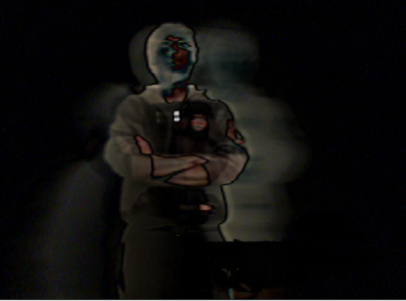
\includegraphics[scale=0.65]{grayscale/grayscale_2}
		\label{fig:grayscale_2}}
		\subfigure[After grayscale filter is applied]{
		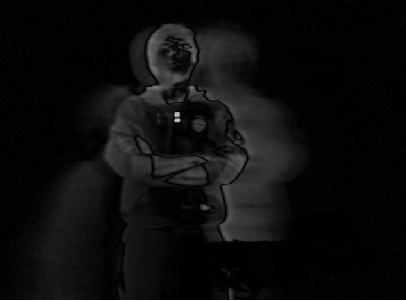
\includegraphics[scale=0.65]{grayscale/grayscale_3}
		\label{fig:grayscale_3}}
		\quad
		\subfigure[After threshold is applied]{
		
\includegraphics[scale=0.65]{threshold/threshold_1}
		\label{fig:threshold_1}}
		\subfigure[After dilation and erosion]{
		
\includegraphics[scale=0.65]{dilate_erode/dilate_erode_1}
		\label{fig:dilate_erode_1}}
		\quad
		\subfigure[After bounding box is drawn]{
		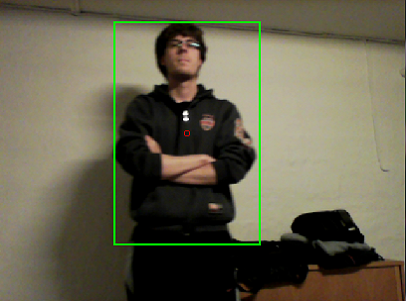
\includegraphics[scale=0.65]{bounding_box/bounding_box_1}
		\label{fig:bounding_box_1}}
		\caption{Object detection example}
		\label{fig:object_detection_example}
	\end{figure}
	
	In conclusion, by applying the steps discussed in this section, we can fairly accurately detect people and their movement in the monitored area.
	
	\subsection{Object Differentiation}
	There will naturally be cases when multiple people will walk through the monitored area and will be captured by the cameras, therefore we must have a way to differentiate between them. This task becomes rather difficult if people are very close to each other, since they will simply be interpreted as one person. However, as long as people are far enough from each other, the task becomes significantly easier. There are multiple ways of differentiating between objects. 
	
	One of them is to simply look at the objects histogram, which gives a graphical representation of the intensity distribution of pixels~\cite{histogram_1}. Since people are usually dressed in different color clothes, we can simply calculate a histogram for every detected person and remember it. Now, every time we receive a new frame and detect a person in it, we go through our previously saved histograms and check whether any of them are the same as our newly detect persons histogram. If there is such histogram, we interpret the person we detected in our new frame as the same person we detected in the last, otherwise, we conclude that we have not detected this person before, thus save his histogram for future reference. The biggest weakness of this approach is that a person's clothes might have different colors from the front and back. Therefore, his histogram calculated while he is facing the camera might be rather different than the histogram of when his back was towards the camera. For this reason, if the person decides to turn around midway, he might be interpreted as a new person - never seen before by the camera - when in fact his frontal or back histogram was already saved. 
	
	Another approach of differentiating between multiple people, and in fact the approach we used in our design, is to simply use the whole frame as a coordinate system and remember the last coordinate of every single detected person. Now, similarly to histogram approach, whenever we detect a new person in the frame, we simply look throughout previously saved coordinates, and if we find that this new person's coordinates is relatively close to some previously saved person's coordinates, we simply interpret him as the same person we detected a second or or few seconds ago, otherwise we see him as a new person. Naturally, we must regularly clear our previously saved coordinates, so that newly arrived person would not simply, by taking a similar path, be interpreted as a person who is no longer in the monitored area. This approach of differentiating between people is is illustrated in Figure~\ref{fig:object_differentiation_example}.
	
\begin{figure}[ht]
		\centering
		\subfigure[One person enters the monitored area]{
		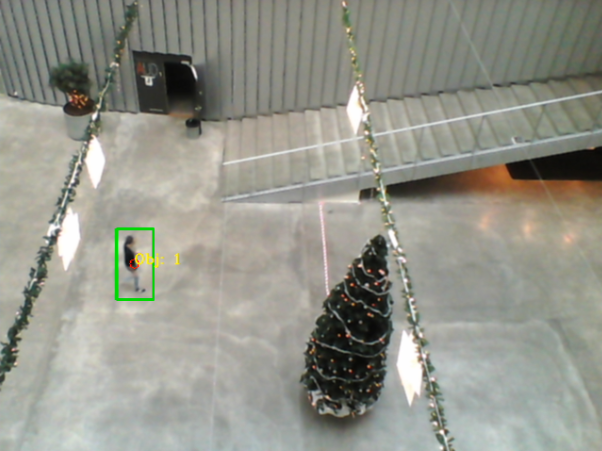
\includegraphics[scale=0.48]{object_differentiation/1}
		\label{fig:object_differentiation_1}}
		\quad
		\subfigure[Second person enters the monitored area]{
		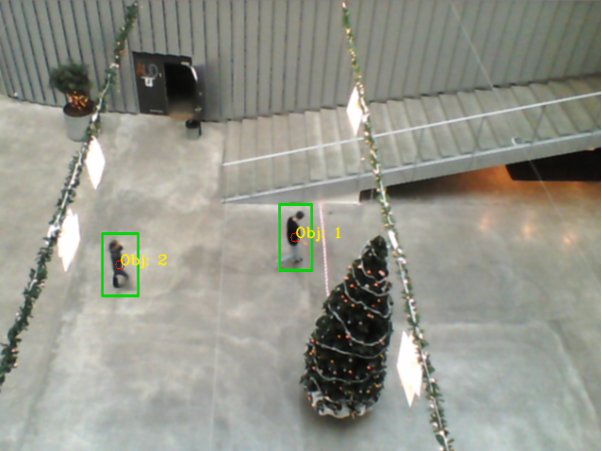
\includegraphics[scale=0.48]{object_differentiation/2}
		\label{fig:object_differentiation_2}}
		\subfigure[Two people continues their walk through the monitored area]{
		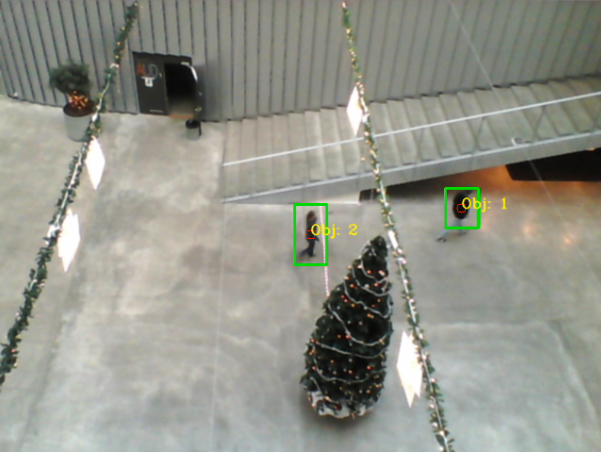
\includegraphics[scale=0.48]{object_differentiation/3}
		\label{fig:object_differentiation_3}}
		\quad
		\subfigure[First person leaves the monitored area]{
		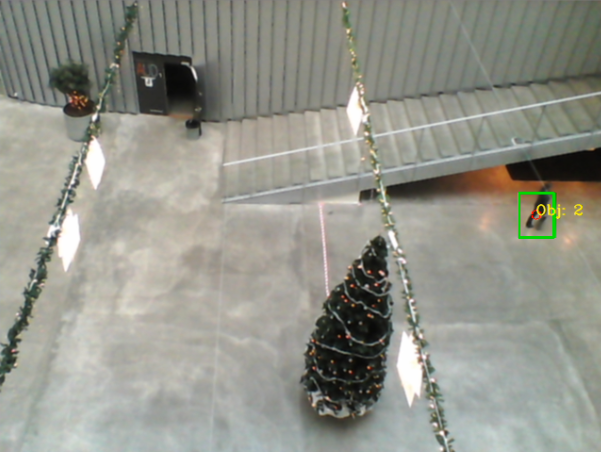
\includegraphics[scale=0.48]{object_differentiation/4}
		\label{fig:object_differentiation_4}}
		\caption{Object differentiation example in the monitored area}
		\label{fig:object_differentiation_example}
	\end{figure}

\section{The Server}
{\color[rgb]{1,0,0} \textbf{\large TODO}}

\section{Prediction}

\subsection{Gathering statistical data}
\label{ssub:statisticaldata}
In addition to storing data about each occupant we also store data about how occupied each section of the recorded image is. The process is simple; we split the image of a room into sections, referred to as cells, and each time an occupant enters a cell the stored activity for the given cell is increased. Each room has a different and independent set of cells. This data tells us which sections of the room are most occupied. We use the activity data to perform predictions about an occupant's future actions using a custom prediction model.

\subsection{Custom prediction model based on HMM}
\label{ssub:designcustomprediction}
We have chosen to build our own prediction model heavily inspired by the hidden Markov model. Each cell in the image is a state where the state transition probability is the likelihood of an occupant moving to an adjacent cell and the output probability is the likelihood of an occupant going to an exit given any current cell. Unlike a regular hidden Markov model, we do not store probability values individually for each state, but rather do the necessary calculations each time a prediction is requested by using the stored activity values of each cell. Additionally, our custom model allows us to take several custom factors into account during calculations. These factors work as a rule set for likely or unlikely occupant actions:
\begin{itemize}
\item An occupant entering a room from a given exit is less likely to exit the room at the given exit.
\item An occupant is more likely to continue moving in his general direction and least likely to return to his previously visited cell.
\item An occupant is more likely to move to the adjacent cell with the highest amount of previous activity.
\item The likelihood of an occupant exiting at a given exit (unless it also serves as the occupant's entrance) is inversely proportional to the direct distance to the given exit, producing a magnet-like effect. 
\end{itemize}
These factors have an influence on a final value of a cell or exit, which is used when calculating each probability. The sum of the probabilities of an occupant moving to each individual exit given a current cell is 100. The cell with the highest probability will be the predicted cell. \\
\begin{figure}
\centering
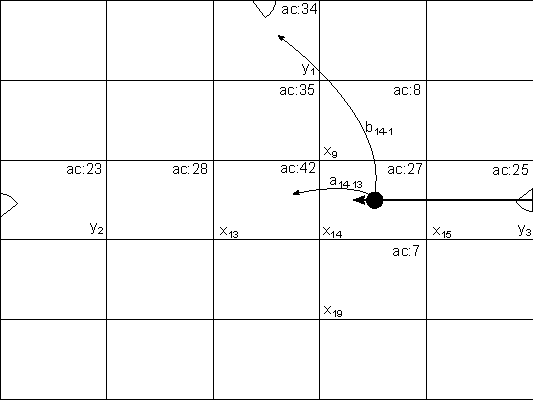
\includegraphics{prediction_figures/custom}
\caption{Applying the custom model to a scenario.}
\label{fig:custom_model}
\end{figure}
Figure \ref{fig:custom_model} shows the custom model translated to a scenario. Each cell contains an identification number, an activity count and a value denoting whether or not the cell is an exit cell. The occupant entered the room at exit \(y_3\) and the current state is \(x_{14}\). \(a_{14-13}\) denotes the state transition probability of the occupant moving from state \(x_{14}\) to state \(x_{13}\). \(b_{14-1}\) denotes the output probability of the occupant ultimately choosing exit \(y_{1}\). Taking our custom rule set into account, the occupant is least likely to exit at \(y_3\) and most likely to continue to \(x_{13}\). Moving to \(x_9\) would increase the probability of the occupant exiting at \(y_{1}\) (\(b_{9-1}\)) significantly.

\section{Android Application}
{\color[rgb]{1,0,0} \textbf{\large TODO}}

\chapter{Implementation}
\label{implementation}
\section{Image Processing}

% Maybe generalize the preference sheet. this was somewhat considered with the server as well.

\subsection{Library}
As non of the group members had any previous experience with image processing, it was quite unrealistic to try to implement all of the image processing techniques needed for this project, and at the same time make them optimized enough, so it could work well and fast on Raspberry Pi computers with limited resources. For this reason the group decided to use an existing image processing library to ease the implementation process. After some research and experiments, we decided go with one of the most popular and well documented libraries called OpenCV~\footnote{OpenCV homepage: \url{http://opencv.org/}.}. OpenCV is an open source computer vision and machine learning software library that has more than 2500 optimized algorithms for image processing. Furthermore, it provides interfaces to multiple popular programming languages, including C\texttt{++}, C, Python and Java.

\subsection{Programming Language}
For determining which programming language to use for image processing on Raspberry Pi computers, skill and preference document (Appendix~\ref{sec:Skill_Preference_Sheet}) was created, where both, ITU and Strathmore University, teams indicated their skill and preference for various programming languages. The two languages that stood out the most were Java and Python, thus to choose one of them, we decided benchmark~\footnote{Code used for benchmarks: Java - \url{http://itu.dk/people/tmis/javatest/}, Python - \url{http://itu.dk/people/tmis/pytest/}.} them in order to compare their performance. The results are presented in the next section.

\subsubsection{Performance Comparison Between Java and Python}
Since the project dealt with a real-time vision application that had to process large amount of frames, we were interested in how fast Java and Python can perform different image processing algorithms. Benchmarks were performed on a laptop~\footnote{Toshiba Satellite L855 Laptop (Intel Core i7-3630QM 2.40 GHZ, 4GB DDR3 1600MHz, Radeon HD7670M 2GB, Windows 7 OS).} and a Raspberry Pi computer~\footnote{Raspberry Pi Computer (ARM1176JZF-S 700MHz, 512 MB memory, Broadcom VideoCore IV graphics, Linux Raspbian OS).} to give some perspective on how much faster a modern laptop is compared to a Raspberry Pi computer.

\begin{itemize}
\item At first we tried to benchmark how fast can Java and Python perform a simple matrix multiplication of two $300 \times 300$ size matrices. The results are illustrated in Figure~\ref{fig:benchmark_multiplication}. We can clearly see that Java was way faster than Python in this benchmark. It took Java less than half of a second to perform the multiplication of two $300 \times 300$ size matrices on a laptop, whereas it took more than 3 seconds to do the same in Python (Figure~\ref{fig:benchmark_1}). Multiplication on a Raspberry Pi computer (Figure~\ref{fig:benchmark_2}) was naturally much slower than on a laptop. Java was again much faster than it's counterpart by dealing with the task in less than 23 seconds, whereas Python was very close to hitting 2 minute mark to accomplish the same task.

In conclusion, as it was expected Java convincingly won the first benchmark.

\begin{figure}[ht]
		\centering
		\subfigure[Time (in seconds) needed to multiply two $300 \times 300$ size matrices in Java and Python on a laptop]{
		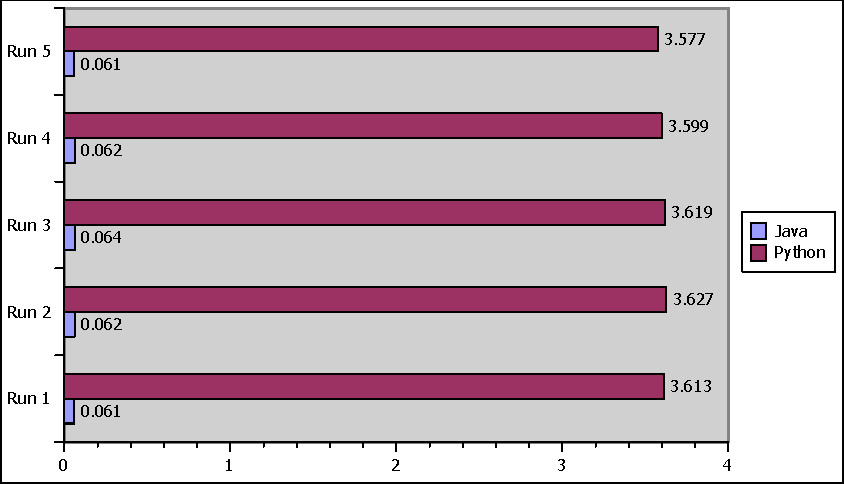
\includegraphics[scale=0.95]{benchmark/benchmark_1}
		\label{fig:benchmark_1}}
		\quad
		\subfigure[Time (in seconds) needed to multiply two $300 \times 300$ size matrices in Java and Python on a Raspberry Pi computer]{
		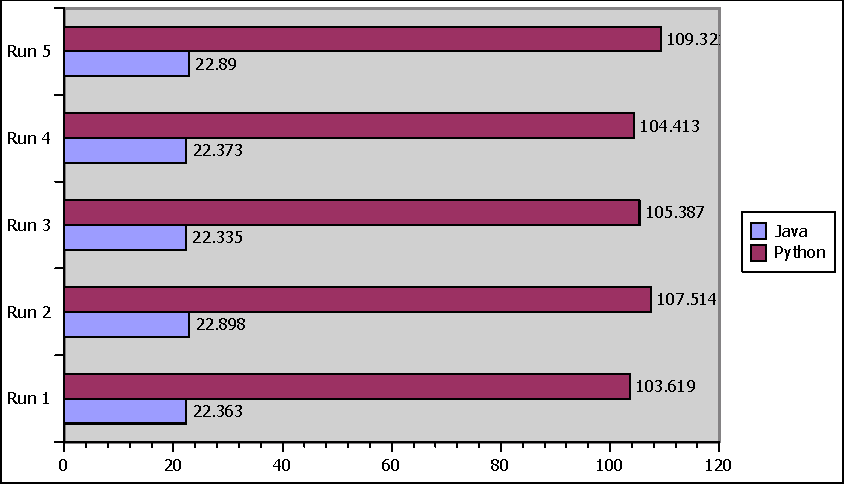
\includegraphics[scale=0.95]{benchmark/benchmark_2}
		\label{fig:benchmark_2}}
		\caption{Benchmark of matrix multiplication of two $300 \times 300$ size matrices}
		\label{fig:benchmark_multiplication}
\end{figure}

\item The second benchmark involved testing how fast Java and Python can perform different image processing algorithms. For this benchmark we used the OpenCV library that we introduced earlier. OpenCV has Java and Python interfaces and all the computations are performed on the native level~\footnote{In C\texttt{++}.}, hence we have some overhead that is equal to a cost of one or several API calls. Consequently, the purpose of this benchmark was to see, which language - Java or Python - has less overhead and can perform API calls faster. 

As we can see in Figure~\ref{fig:benchmark_image_processing}, the difference between Java and Python in this benchmark was rather small on both, laptop~\ref{fig:benchmark_3} and Raspberry Pi computer~\ref{fig:benchmark_4}. This was rather surprising at first, since Java had a big edge in the first benchmark. One can speculate that Python's interface to OpenCV library has been implemented in a more efficient and optimized way than Java's, thus the outcome. In general, the difference was only in terms of a few milliseconds, however, it was a good enough reason for us to choose Python's interface to OpenCV library for image processing part in this project.

\begin{figure}[ht]
		\centering
		\subfigure[Time (in seconds) needed to process images in Java and Python on a laptop]{
		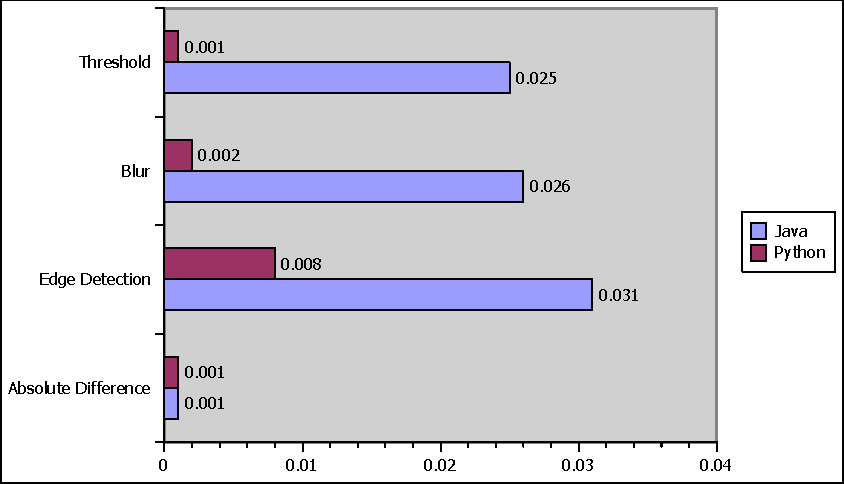
\includegraphics[scale=0.95]{benchmark/benchmark_3}
		\label{fig:benchmark_3}}
		\quad
		\subfigure[Time (in seconds) needed to process images in Java and Python on a Raspberry Pi computer]{
		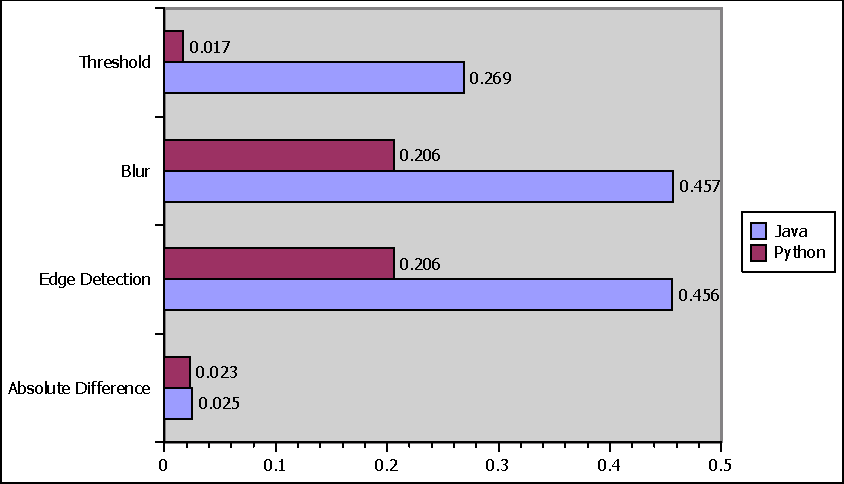
\includegraphics[scale=0.95]{benchmark/benchmark_4}
		\label{fig:benchmark_4}}
		\caption{Benchmark of image processing}
		\label{fig:benchmark_image_processing}
\end{figure}
\end{itemize}

\section{The Server}
Server...

\chapter{Evaluation}
\label{evaluation}
To evaluate the final system, we did a quantitative evaluation based on experimentation. We set up several scenarios taking place at the ITU. The results of each scenario are presented and interpreted below. Due to the issue mentioned in the first scenario we chose to test the prediction implementation separately.

\section{Scenario 1}
\label{sec:scen1}
\textit{\textbf{Purpose.}} The purpose of this scenario is to test if the Raspberry Pi computers correctly analyze the image and send the correct data to the server.

\textit{\textbf{Setup.}} For this experiment, we have set up three web cameras each connected to a Raspberry Pi computer and recording the Atrium of the ITU from the 4th floor. This is illustrated in Figure~\ref{fig:evaluation_setup}.

\begin{figure}[htb]
	\centering
	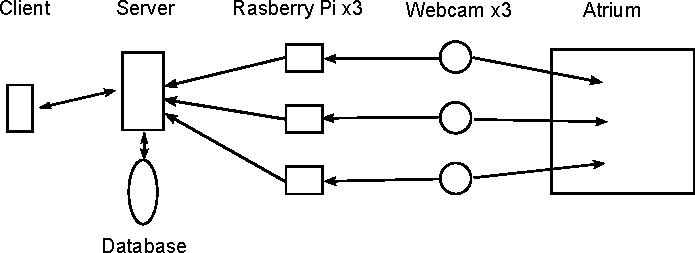
\includegraphics[scale=0.85]{evaluation/evaluation_setup}
	\caption{Experimental Setup}
	\label{fig:evaluation_setup}
\end{figure}

First, three exit areas are manually set in one area by sending requests to the server containing the coordinates of the desired exit points. 

The experiment starts with a single person walking across the monitored areas. We perform a probability request by providing a room id and the id of the detected person, which is stored in the database. The Raspberry Pi sends data about the person's position and room to the server which stores it in the database.

\textit{\textbf{Results.}}
\begin{enumerate}
\item The coordinates of the person are calculated and stored correctly while the id of the object is mistranslated and is stored incorrectly. 
\item The server returns a set of probabilities to each exit, which are not very accurate.
\end{enumerate}

\textit{\textbf{Interpretation.}} The outcome of result 1 indicates that the server does not maintain a link between each coordinate, thus, the complete path of the person is not stored. This is crucial since the data about a person's path is essential in calculating probabilities. This is shown in the outcome of result 2 containing inaccurate probabilities. This is because the lack of path information prevents the probability calculations from using the previous position of an occupant, as well as the entrance area of the occupant. Ultimately, this made us choose to test the prediction model in a separate environment. The tests are described in Section~\ref{eval_prediction}.

\section{Scenario 2}
\textit{\textbf{Purpose.}} The purpose of this scenario is to test the image analysis when multiple people are present in the monitored area.

\textit{\textbf{Setup.}} The setup of this experiment is exactly the same as in Scenario~\ref{sec:scen1}.

The experiment starts with multiple people entering and exiting the monitored area.

\textit{\textbf{Results.}}
\begin{enumerate}
\item Several people are moving while keeping a distance of 2 or more meters of each other and are interpreted as separate occupants with different ids.
\item Several people are moving while keeping a distance of less than 2 meters of each other and are interpreted as one occupant with the same id (Figure~\ref{fig:evaluation_1}).
\item Two people are entering the monitored area and are initially interpreted as separate occupants. They intersect and split and are interpreted as new occupants.
\end{enumerate}

\textit{\textbf{Interpretation.}} The outcome of result 2 and 3 is partly due to the camera placement and because the differentiation of the occupants is only based on the positions.

\begin{figure}[htb]
	\centering
	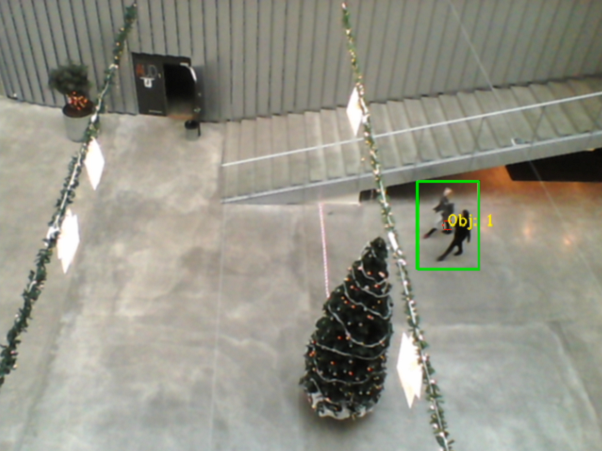
\includegraphics[scale=0.82]{evaluation/evaluation_1}
	\caption{Problem of two people walking too close to each other}
	\label{fig:evaluation_1}
\end{figure}

\section{Prediction model}
\label{eval_prediction}
Due to the issue mentioned in section \ref{sec:scen1}, we continued the testing of the prediction model in a separate program allowing for easy setup of a desired scenario testing various aspects of the prediction model. The program is implemented in C\# and uses the same logic as the Java implementation. Figure \ref{fig:pred_c} shows an image of the program where each cell is marked with the activity value. 

\textit{\textbf{Purpose.}} The purpose of this setup is to test whether the implemented rule sets have an effect.
\begin{figure}[htb]
	\centering
	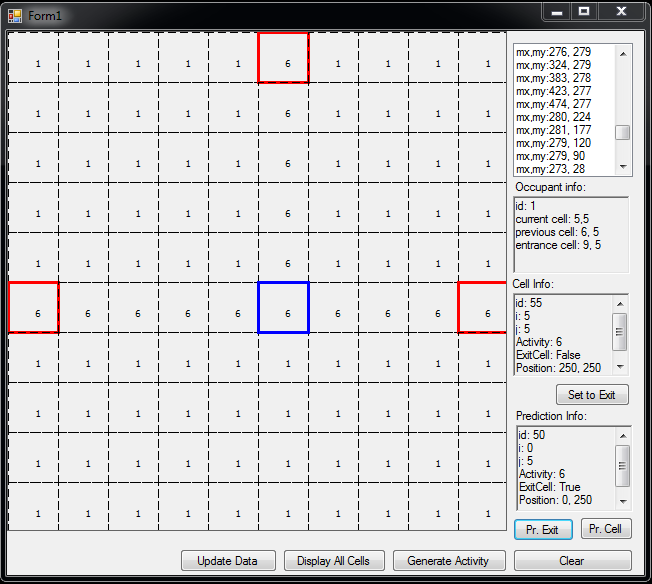
\includegraphics[scale=0.82]{prediction_figures/prediction_csharp}
	\caption{Screenshot of the prediction test program.}
	\label{fig:pred_c}
\end{figure}

\textit{\textbf{Setup.}} The image depicts a scenario where the occupant entered at the right exit and moving left. He is currently positioned at the blue square. By pressing the "Pr. Exit" button the program will perform the calculation. 

\textit{\textbf{Results.}} The left cell is the predicted exit. The probabilities for each exit are only printed to the console in the test program. The results are:
\begin{verbatim}
    Exit at: 0 , 5 , prob=0,3576
    Exit at: 5 , 0 , prob=0,3494
    Exit at: 9 , 5 , prob=0,2930
\end{verbatim}

\textit{\textbf{Interpretation.}} Since each activity value is the same along the paths to each exit, the rules must have had an effect. The occupant is most likely to exit to the left because he came from the right. He is least likely to exit to the right even though he is positioned closer because this exit serves as his entrance. Moving the occupant one cell to the left increases the probability that he will exit to the left to 0,4935. This is intended as the distance to the left exit decreases. Increasing the activity value in the cells along the path to the topmost exit to 7 increase the probability to the topmost exit to 0,3607, making it the predicted exit when the occupant is positioned at the original location.

\chapter{Collaboration}
\label{collaboration}
This chapter deals with the collaboration and process in the project. First we introduce some theory on project management and global collaboration. In the next step we report our project work: We introduce the project team, the initial situation and present the chosen project management approach, methods and tools. In addition we evaluate the collaboration tools we used in the project. Finally, we cover the issues we had to face during the project. These include progress issues, issues with the used project management techniques and collaboration issues. We analyze the collaboration issues based on the previous introduced theory. Furthermore we reflect on the process and collaboration and explain our learning outcomes.

%---

\section{Theory}

\subsection{Project management}

There are several approaches how you can perform project management for software development projects. It is often distinguished between the traditional approach and the agile approach in project management.

The traditional approach in project management is dividing the project into distinguished phases, which are planned in advance. The phases are run sequentially. Theoretically, once a phase is complete it will not be revisited. This structure is also known as waterfall model in software development.
The traditional approach plans the project in the beginning. All requirements and ressources are collected and planned in the beginning of the project to build up a project plan, which containes a detailed project tasks and milestones. These pre-planned project tasks are then worked off during the project. The project manager can keep track and report the progress of the project by comparing planned and actual progress.

The problem with this traditional approach is that it is not very flexible for unpredictable events. Furthermore, clients are often unable to state all requirements in the beginning. A change of a requirement or the adding of additional requirements during the project can have a major impact on the project plan and is often embedded in some kind of change management process.

The agile approach is in general more flexible than the traditional approach, especially when it comes to requirements and unpredictable events. The idea of an agile approach is to have many iterative planning and development cycles. The approach supports quick results, which are constantly improved by involve the client actively in the project progress.

An agile approach is not a completely pre-planned process like in the traditional approach. In software development projects an agile approach is preferred due to it's advantages. A popular agile project management framework is Scrum.

An agile approach requires a strong collaboration between the project team members and healthy communication. It is also essential, that the project team members have the needed competencies and that the users and executives support the project \todo{Add reference}.

\subsection{Global collaboration} \todo{TODO}
Globally-distributed projects are becoming more popular for large software systems. The advantages of globally-distributed projects are that the

Reasons are on the one hand to outsource 

In the paper “Managing cross-cultural communication in multicultural construction project teams: The case of Kenya and UK”  from E.G. Ochieng and A.D.F. Price

	\begin{itemize}
		\item Trust
		\item Individualism
		\item Power distance
	\end{itemize}

%---

\section{Background information of the Project Team}
The project team consists of two groups of students. One group is from Strathmore University located in Nairobi (Kenya). The other group is from the IT University (ITU) in Copenhagen (Denmark). The project team agreed on to name the two groups "Team Kenya" for the student group from Strathmore University and "Team ITU" for the student group from ITU. This helped to address each group in meeting reports, emails and conversations.

In the following paragraphs the background information for this project from both groups are introduced. The information explains the motivation and contribution of each group in the project and is used in arguments for why certain decisions were made and issues arise.


\subsection{Team ITU}
Team ITU started with four members, which are all in the Masters programme "Software Development and Technology (Software Engineering)" of the ITU\footnote{In the beginning there were five members, but one left the project after two weeks, because he changed to another project and project team. This did not have an impact on the work as it was in the early stage of the project.}. The members are from three different countries: Lithuania, Germany and Denmark\footnote{Although there are minor differences between the nationalities, which could have an influence on the team work, we will not go into this, because it is out of scope for this report.}. The communication language within Team ITU is English, which is not the mother tongue of any of the members. Two of the members of Team ITU already collected some negative experience with previous global collaboration projects and were not very interested on a global collaboration. They experience that the other groups in their previous global collaboration projects did not put much effort into the projects, so that they and their local team had all the workload. The members of Team ITU met each other the first time on the 27.8.2013.

The students of Team ITU have to complete the project under the course "Global Software Development Project", which is mandatory for their masters programme. The requirements and deadlines for the project are given in the course base from ITU (reference\todo{Link to the course base}) and by the advisor of the project. The course is rated with 15 ECTS points, which corresponds to approximately 20 hours per week per student. The students of Team ITU have to hand in this report as a mandatory requirement.

As the course for the Team ITU started in late August and the project team and topic was already known, Team ITU already started with the project work before Team Kenya. Team ITU and their advisor did not know when they would get the contact details from the student group in Kenya, so the advisor recommended already initializing the project and doing some research and thoughts on the project.

At the beginning Team ITU had received a different project topic by the advisor. The topic of the first project was "Vector Shooter"\footnote{In this project a game had to be developed, in which the calculation of a vector - based on an image - had to be made. The image should contain a person, who uses his hands to demonstrate a vector by taking a position like he uses a bow and arrow. The requirement was to use webcams, to capture the image, and to use RaspberryPis to detect the hands of the person and to calculate the vector. Furthermore, an Android application should be included in the program.}. Team ITU put some thoughts into the project and spent time on defining the program, which they wanted to develop\footnote{Team ITU planned to develop an individual cannon game with an appropriate concept for a global collaboration project.}.

After three weeks the advisor had to change the topic of the project due to the collaboration with Strathmore University. Only one student from the Strathmore University was interested on the project "Vector Shooter". Team ITU could have spent time and effort in convincing the other students from Strathmore University to do the project "Vector Shooter". Despite frustration, in consideration of the given deadline of the course and on recommendation of the advisor, Team ITU decided to not take this option.

Team ITU received the project topic and the contact details of the members of Team Kenya on the 17.9.2013. So the collaboration between the student groups did not start before this date.


\subsection{Team Kenya}

In the beginning Team Kenya consists of three members, which are all in the Masters programme "Telecommunication and Innovation" of the Strathmore University. The members are all from Kenya. The official languages in Kenya are English and Swahili. The members of Team Kenya met each other the first time on the 1.10.2013 (--> Appendix \ref{app:appendixB}: \hyperlink{GSD20131001.1}{Global Meeting Report 1.10.2013 Page 1}). One member had to leave the group in the last third of the project due to workload of other projects and obligations (--> Appendix \ref{app:appendixB}: \hyperlink{GSD20131126.2}{Global Meeting Report 26.11.2013 Page 2}).

The department, which is responsible for the masters programme "Telecommunication and Innovation", wants to convince the school management from Strathmore University to invest into the technology and idea of the project to improve environmental conservation. Therefore this collaboration project was initiated. (--> Appendix \ref{app:appendixB}: \hyperlink{GSD20131203.2}{Global Meeting Report 3.12.2013 Page 2}) \todo{Maybe in the Introduction-Context Part?}.

For the students from Team Kenya the project is not included in any mandatory course and is completely voluntarily. The students from Team Kenya spend their free time on this project. There are no mandatory requirements or deadlines, which the Kenyan students have to achieve, except that they have to create documentation for their advisor to prove the progress of the project (--> Appendix \ref{app:appendixB}: \hyperlink{GSD20131119.2}{Global Meeting Report 19.11.2013 Page 2}). The motivation for the Kenyan students to participate in this project is on the one hand to support the environmental thought and on the other hand to use this project work as basis for their master thesis (Email 10.12.2013 \todo{Add refernce}).

%---

\section{Project Management}

\subsection{Approach}

As the course for the team ITU started in late August and the project team was already known, Team ITU already started with a project management technique. This was already established when Team Kenya got into the project.

Team ITU chose an agile project management approach, because it is more flexible, which was important due to the fact, that Team ITU did not knew the student group from Strathmore University neither their skills nor their requirements on this project. Moreover an agile project management approach is known for being more suitable for software development projects (*TODO: reference*\todo{Find reference}).

Team ITU planned to merge Team Kenya into their project management approach, because they did not come up with a different approach on how to organise the project. Team ITU asked several times for feedback or other suggestions according to project management methods and tools, but Team Kenya did not react at all or agreed with the suggestions of Team ITU. So Team ITU assumed that Team Kenya is fine with the project mangement approach. In general Team Kenya was very reticent in project management topics, although one student from Team Kenya seemed to be very interested in the project management and global collaboration challenges (--> Appendix \ref{sec:Motivation_Sheet}). The reason for this could be, that Team Kenya had not much time to spend on the project. In the end it also turned out, that the one kenyan student, who was the most interested in project management and global collaboration, left the project due to other obligations.

Team ITU considered introducing Scrum to the project. However, due to the inexperience and non-knowledge about this framework in both teams, this idea has been dropped. For Scrum it is necessary that every project team member knows the concept. Thus, each team member would need to learn Scrum, which in turn would have taken ressources from the implementation.

%---

\subsection{Project Organization}

\subsubsection{Timeline}
Team Kenya agreed on to go with the deadlines from Team ITU as they do not have to meet any deadlines. (--> Appendix \ref{app:appendixB}: \hyperlink{GSD20131024.1}{Global Meeting Report 24.10.2013 Page 1})

\subsubsection{Project Team and Roles}
Each member of the project team created a member profile to introduce themselves, which are attached in the Appendix \ref{sec:member_profiles}.

The members of Team ITU split up the tasks, such that different kind of roles arose. The roles were not set in the beginning, but emerged during the progress of the project. They define the major responsibilities. This does not

\textbf{Collaboration master}

\textbf{Server Developer}

\textbf{Image Processing Developer}

\textbf{Prediction Model Developer}

\textbf{Team Kenya/Android Application Developers}


%---

\subsection{Project Management Tools and Methods}

\subsubsection {Member profiles}
Team ITU suggested to come up with some member profiles of each project team member to introduce each other in the beginning of the project. The intention of the member profiles was to set the first steps for building up trust within the distributed project team. The project team members could recognise the members as individual persons with own personalities and different backgrounds in the beginning. The profile members should also preclude misunderstandings, for example according to the genders and how to address a person.

One member of Team Kenya followed the suggestion in the beginning. The other two members provided their member profiles three weeks after Team ITU reiterated the request.

Because Team ITU did not receive the member profiles of all students from Team Kenya in the beginning, a first disappointment on the side of Team ITU could be noted. Team ITU already waited since end of august to meet the Kenyan group, with whom they supposed to work with. There was high curiosity on the side of Team ITU, which was not satisfied by Team Kenya. This probably already led to a higher mistrust, as two members from Team ITU, which already collected some negative experience with previous global collaboration projects, felt reassured.

\subsubsection {Introduction and Kick-Off meeting}

\subsubsection {Skill-/Preference- and Motivation-Sheet}
To see where the strengths, weaknesses and motivations within the project team are Team ITU came up with a Skill-/Preference-Sheet and Motivation-Sheet. The Skill- and Preference-Sheet focusses on the technical concerns like programming languages, version control tool, database- and other technologies. So when a skill in a technology is purely pronounced within the project team, the most preferred technologies can be considered. The Motivation-Sheet, on the other hand, focusses more on the different project work tasks and topics. With this information the roles within the project can be split up, so that every member is the most satisfied and therefore more motivated.

Every project team member was encouraged to fill out these tables. The results can be seen in the Appendix \ref{sec:Skill_Preference_Sheet} and \ref{sec:Motivation_Sheet}.

The outcome of these tables also influenced some decisions in the project. For example, the decision of which programming languages Team ITU choose to benchmark was based on this (*reference*)\todo{Add reference}. Also the choice of database technology and which version control system to use for the source code is based on the Skill-/Preference-Sheet. It also pointed out the possible roles of each project team member within the project (*reference*)\todo{Add reference}.

In the result it can be noticed that image processing, prediction models and RaspberryPis were quite unknown amongst the project team members. So each project team member was encouraged to do some research on these topics in the beginning.

\subsubsection{"Out-of-Office"-Calendar}

Because every project team member had different obligations besides the project, Team ITU came up with an "Out of Office"-Calendar, in which every project team member could publish for example exams, other hand-ins or other unavailability. The motivation of this calendar was to allow for better planning of meetings and assignments during the project. The problem was that no one really looked into this calendar except in the beginning of the project or when a certain issue aroused. The "Out-of-Office"-Calendar can be seen in the Appendix \ref{sec:Calendar}.

So it was noticed by Team ITU that Team Kenya as well as Team ITU had some exams in October. This influenced the project plan according to when to probably start the implementation phase. In the first half of November Team Kenya had a second exam phase. This was not correctly mentioned in the calendar, so Team ITU was not aware of this situation in the beginning. Team ITU got informed of the exam phase by Team Kenya in a meeting, when Team Kenya excused themselves for the non-fulfillment of agreed assignments (--> Appendix \ref{app:appendixB}: \hyperlink{GSD20131112.2}{Global Meeting Report 12.11.2013 Page 2}). This led to amazement and disappointment on the side of Team ITU. Team ITU wondered why Team Kenya even agreed on the assignments the week before, when they knew that they probably do not have the time to fulfill these assignments. Team ITU expected that Team Kenya communicates such situations before they happen.

\subsubsection{Milestone plan}
Team ITU chose to create a very rough milestone plan to have an eye on the deadline given by ITU. A detailed milestone plan would contradict the idea of the agile project management approach. Team ITU did not know Team Kenya, their skills and requirements in the beginning and a detailed milestone plan probably would have been rescheduled several times. In the milestone plan Team ITU roughly pointed out when they want to be done with each phase of the project.

The following milestones where set in the beginning of the project.

\begin{table}[htb]
	\centering
	\begin{tabular}{ |  p{4cm} |  p{6cm} | l | l |}
    		\hline
   		Milestone & Description & Planned & Achieved \\ \hline
    		First Global Meeting & Introduction session with Team Kenya to get to know each other and sharing requirements and expectations of the project & 01.10.2013 & 01.10.2013 \\ \hline
    		Final definition of Requirements and Roles & Get all the main requirements together and splitting up the project tasks & 31.10.2013 & 03.12.2013 \\ \hline
    		Finishing Prototype & A complete prototype of the product & 01.12.2013 & 15.12.2013\\ \hline
		Report & A complete final report of the project & 13.12.2013 & 16.12.2013\\ \hline
	\end{tabular}
	\caption{Milestone Plan}
	\label{tab:milestones_table}
\end{table}

As it can be seen in table \ref{tab:milestones_table} the planned milestones were mostly not achieved in time. The most significant difference between a planned and a achieved date can be seen at the second and third milestone, which contained a final defintion of requirments and roles and the development of a prototype. The reason for this is on the one hand that Team ITU was too optimisitic in the planning process of these milestones, as they assumed that the members of Team Kenya have the same work pace and working experience like they have.

Furthermore the milestone plan was not properly introduced and discussed with Team Kenya. But that is because Team Kenya did not show much interest and their response time was very slow, especially in the first two months of the project. On the other hand Team ITU could not encourage Team Kenya enough to do their part of the project in time or the results were not satisfactory enough, such that Team ITU could work with it. In consequence several iterations and new requests had to be made from Team ITU to Team Kenya, which slowed down the project progress a lot. Team ITU was to patient in the end, because they still hoped that Team Kenya will get a better drive after their exam period as Team Kenya make Team ITU believe.

Figure~\ref{fig:milestones} shows the milestone plan, which was planned in the beginning of the project.

	\begin{figure}[htb]
		\centering
		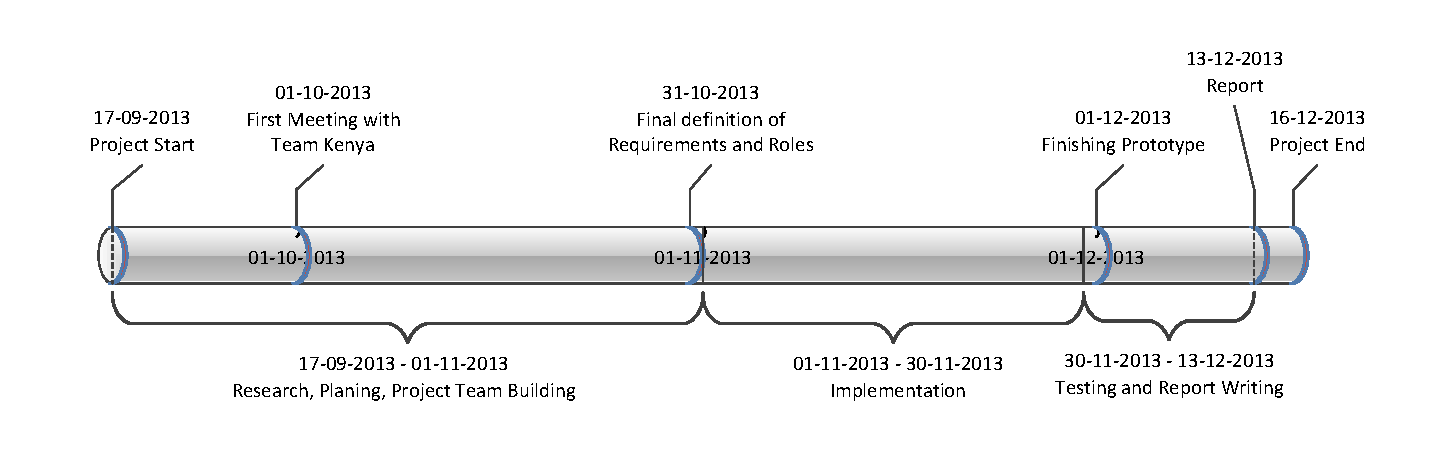
\includegraphics[scale=0.7]{collaboration/Milestones}
		\caption{Milestone Timeline}
		\label{fig:milestones}
	\end{figure}

The milestone plan was mostly a guideline for Team ITU, because they had a deadline in contrast to Team Kenya. Team ITU shared the planed dates for half of the milestones with Team Kenya as they agreed to go with the deadlines from Team ITU. (--> Appendix \ref{app:appendixB}: \hyperlink{GSD20131024.1}{Global Meeting Report 24.10.2013 Page 1}) These shared milestones were according to when to finish the prototype and when to hand-in the mandatory final report.

\subsubsection{Internal weekly meeting (Jour-Fixe)}
Team ITU agreed on having an internal weekly meeting to update each other on the current progress, to discuss occuring topics, make decissions, work together and assign each other new assignments till the next meeting. Furthermore Team ITU also met with their advisor to check if they are on the right track. The concept of the weekly meeting equates to the concept of a Jour Fixe \todo{Find reference} or a Daily Scrum \todo{Find reference}.

There was a constant agenda for the meeting:

	\begin{enumerate}
		\item Status update of each team member
			\begin{enumerate}
				\item What has each group done during the past week according to the project?
				\item Which achievements were made?	
				\item Which problems occurred?
				\item Any other news
			\end{enumerate}
		\item Discussions and Decisions (the topics in this section varied weekly according to the current progress)
		\item Meeting with advisor	
		\item Assignments
	\end{enumerate}

This constant agenda gave some structure to the project. The team members knew what to expect from the meeting and where they can place their concerns.

The members of Team ITU were mostly fully represented in the internal weekly meeting. 

\subsubsection {Global weekly meeting (Jour-Fixe)}
Team Kenya and Team ITU agreed on having a weekly Skype-Meeting (*reference*\todo{Add reference}) to update each other on the current progress, to discuss occurring topics, make decisions and assign each other new assignments till the next meeting, just like the weekly internal meeting. The meeting took place every Tuesday afternoon/evening. According to a Doodle-Survey (*reference*\todo{Add reference}) all project team members could reserve this time for the project meeting.

Each group could make a suggestion for the Agenda, but Team Kenya never used this opportunity. Therefore only Team ITU prepared an agenda, which was structured in the following way:

	\begin{enumerate}
		\item Status update of each group
			\begin{enumerate}
				\item What has each group done during the past week according to the project?
				\item Which achievements were made?	
				\item Which problems occurred?
				\item Any other news
			\end{enumerate}
		\item Discussions and Decisions (the topics in this section varied weekly according to the current progress)
		\item Assignments
	\end{enumerate}

It can be noted, that the structure for the agenda of the global meeting is similar to the agenda of the internal meeting. This is because the structure was already proofed by Team ITU before the global colaboration started and was considered to be suitable by all members from Team ITU. Although it was offered to Team Kenya, they never made alterations to the agenda.

After the first few meetings Team Kenya and Team ITU agreed to prepare the status update in advance, because it took quite a while for each group to present their status updates in the Skype chat. Unfortunately Team Kenya did not comply with this agreement except in the last meeting, where none of the Kenyans could attend due to other obligations or internet connection problems (Table~\ref{tab:global_meetings}).

\begin{table}[htb]
	\centering
	\begin{tabular}{ | l |  p{2.5cm} |  p{2.5cm} |  p{3cm} |  p{3cm} |}
    		\hline
   		Global Meetings & Attendance Team ITU &  Attendance Team Kenya & Prepared Status update Team ITU & Prepared Status update Team Kenya\\ \hline
    		01.10.2013 & 4 & 1 & no & no \\ \hline
    		24.10.2013 & 4 & 2 & no & no \\ \hline
    		31.10.2013 & 3 & 2 & no & no \\ \hline
    		12.11.2013 & 4 & 2 & no & no \\ \hline
    		19.11.2013 & 4 & 2 & yes & no \\ \hline
    		26.11.2013 & 4 & 1 & yes & no \\ \hline
    		03.12.2013 & 3 & 1 & yes & no \\ \hline
    		10.12.2013 & 4 & 0 & yes & yes \\ \hline
	\end{tabular}
	\caption{Attendance and prepared status updates of the global meetings}
	\label{tab:global_meetings}
\end{table}

As it can been seen in Table~\ref{tab:global_meetings} almost every meeting took place. Team ITU was always in the majority. The attendance from Team Kenya was low mostly due to other obligations and internet connection problems.

\subsubsection {Meeting reports}

For every internal and global weekly meeting Team ITU wrote a meeting report. These meeting report documents all updates, news, discussions, decisions and assignments, which were discussed in the meetings. After publishing the meeting report, each project team member had the chance to correct wrong information or add missing information for the next couple of days. Afterwards the information and assignments in the meeting report were binding.

Project team members which could not attend the meeting had the chance to be updated with all necessary information. The report also serves to confirm the content of the meeting. Furthermore, the report is a source the team members can rely on. For example in case it comes to false allegations against a team member, the report could be used as a proof. The meeting report is also a reminder on the agreed tasks.

Team ITU expected that the agreed assignments were done or at least initiated to the next meeting. Since this never happened on the side of Team Kenya in the beginning, Team ITU started to put some deadlines on the most important assignments. But even those assignments were mostly not done in time, satisfactory or done at all, although Team ITU got specific confirmation by email on the published meeting report or no disagreement on the meeting report from Team Kenya.

This lack of collaboration and passive attitude of Team Kenya frustrated the members of Team ITU a lot, such that the motivation of Team ITU on collaborating with Team Kenya was gone by the half of the project. Also the expectations towards Team Kenya changed much lower expectations than in the beginning.

\subsubsection {Time recording}
Time recording is a quite popular tool amongst consultancies. Consultants record their times to keep track of project work they are performing for different customers. Based on this recorded times correct invoicing can me ensured. Some Human Resources Departments also use time recording to keep track of the presence of their employees. But it also can be used for other purposes.

Team ITU decided to record the time they spend on each part of the project. This time recording data helped to evaluate the spended time on a topic for each team member and for the whole group. This information can be a motivator in those situations, where it seems that no progress is done. If no visible progress was made within the project, the information of spended hours made it less frustrating. Furthermore, it also can encourage members to work on the project by either comparing themselves to other team members or assess whether the time they spend is appropriate. This worked out for Team ITU, because the attitude towards the project of each member was similar.

The only challenge of this tool is that you have to remember to record your time. To make it more easy Team ITU used a time recording software (See in section \ref{sec:timeRecTool}).

\begin{table}[htb]
	\centering
	\begin{tabular}{ |  p{3,5cm} |  p{2cm} |  p{2cm} |  p{2cm} |  p{2cm} |  p{2cm} |  p{2cm}|}
    		\hline
   		Project Parts & September & October & November & December & Total\\ \hline
    		Lectures/Advisory Meetings & 4 \% & 12\% & 5\% & 3\% & 5\% \\ \hline
    		Reasearch & 58\% & 29\% & 11\% & 3\% & 16\% \\ \hline
		Internal Collaboration & 9\% & 33\% & 20\% & 15\% & 20\%\\ \hline
    		Global Collaboration & 1\% & 23\% & 13\% & 4\% & 11\%\\ \hline
    		Implementation and Testing & 0\% & 0\% & 39\% & 15\% & 23\% \\ \hline
    		Report & 17\% & 1\%  & 8\% & 59\% & 22\% \\ \hline
 		Other & 11\% & 2\% & 4\% & 1\% & 3\%\\ \hline
	\end{tabular}
	\caption{Results of the time recording for the Project "Occupancy Analyzer". The table shows the ratio of hours spend for each project part for each month. In addition the table also contains the ratio of hours for each project part for the whole duration of the project. The data is based on the recorded times in the Time Recording Software "Toggl" between the 17.9.2013 and 13.12.2013.}
	\label{tab:timeRecResults}
\end{table}

Team ITU was also interested in the result of the total hours spend in each project part in the end of the project. The results\footnote{Note that these results contain approximately values due to the fact that not every time was recorded} can be seen in Table \ref{tab:timeRecResults}.

It can be noticed that research was a main task in the first half of the project, while in the second half of the project the focus was mostly on the implementation. This approximately conforms with the planned milestone plan in Table \ref{tab:milestones_table}.

The amount for internal collaboration activities was more or less constant. An higher workload can be noticed in October. The same pattern can be seen on the global collaboration work. Also here is the highest work load in October. This is probably because the most communication and initialization according collaboration had to be set in the beginning.

Team ITU did not suggest this tool for the whole project team, because they had the feeling that it would be an overload for Team Kenya, which already had troubled to deliver progress within the project.On the other hand the result would have been very intersting and informing for Team ITU, as they presume Team Kenya does not put any effort into the project.

\subsubsection {Surveys}

%---

\subsection{Collaboration Tools}

\subsubsection {Communication}
	\begin{itemize}
		\item Skype (excluding Google Hangout)
		\item Email
	\end{itemize}
\subsubsection {Sharing}
	\begin{itemize}
		\item Google Drive (excluding Skydrive)
		\item Github
	\end{itemize}
\subsubsection {Time recording}
\label{sec:timeRecTool}
	\begin{itemize}
		\item Toggl (excluding Excel)
	\end{itemize}

%---


\section{Project Issues}

\subsection{Collaboration Issues}
%The issues and how you responded to them

	\begin{itemize}

		\item Illusion of the project work and project team
		\item Failure to comply with the assignments
		\item Communication
		\item Lack of skills
		\item Other exams/hand-ins
		\item Differing requirements
		\item Attendence of meetings
		\item Equipment
		\item Prejudice
	\end{itemize}

%---

\section{Hypothetical Scenarios}
%Relevant hypothetical scenarios

	\begin{itemize}

		\item Assignments
		\item Communication
		\item Requirements
		\item Organisation by the universities (Requirments, clarification, )
	\end{itemize}


\chapter{Conclusion}
\label{conclusion}
Despite the collaboration difficulties and mitigations mentioned throughout section \ref{collaboration}, we succeeded in designing and implementing a system to solve the overall problem regarding occupancy analysis. The system makes use of the lowcost computational devices, Raspberry Pis, to perform the image analysis, supported by a central server handling database- and client communication. We solved the problem regarding the visual conditions of the image by using the running average approach to dynamically update the background image. The prediction problem was solved by building and integrating our own custom prediction model into the server. The model is inspired by the hidden Markov model and makes use of historical data about occupant activity in a room. 

While the final system allows a user to detect occupants and predict their future actions, the evaluation revealed some flaws causing a significant impact. In order to perfect our solution we propose several future improvements: 
\begin{itemize}
\item The coordinates of each occupant needs to be stored correctly.
\item The occupant detection should be able to distinguish between occupants moving close to each other.
\item The server could store a list of occupants having recently resided in a room. This would simplify the process of displaying the relevant occupants in the Android application as well as increasing the relevance of requesting predictions.
\item The prediction of an occupant should be more flexible, allowing for different meaningful requests. A request about predicting every present occupant at a time with corresponding probabilities could be supported. 
\item The server could use the stored activity values for different tasks, such as analysing the most occupied areas of a room. This information could be used for advertisement placement.
\end{itemize}

\begin{thebibliography}{}
%% Introduction %%

% Related Work %
% Image Processing %
\bibitem{simple_background_subtraction} Y. Benezeth, P.-M. Jodoin, B. Emile, H. Laurent \& C. Rosenberger. October 2012. \emph{Comparative Study of Background Subtraction Algorithms}, pp. 5-6.

\bibitem{jog_halbe} Aditi Job \& Shirish Halbe. October 2012. \emph{Multiple Objects Tracking using CAMshift Algorithm in Open CV}, pp. 41-46.

% Prediction %
\bibitem{gellert} Gellert, A. \& Vintan, L., 2006, \emph{Person Movement Prediction Using Hidden Markov Models}, Computer Science Department, University of Sibiu, \url{http://webspace.ulbsibiu.ro/arpad.gellert/html/SIC_HMM.pdf}.

\bibitem{ashbrook} Ashbrook, D. \& Starner, T., \emph{Using GPS to Learn Significant Locations and Predict Movement Across Multiple Users}, Georgia Institute of Technology, \url{http://www.cc.gatech.edu/~thad/p/journal/using-gps-to-learn-significant-locations.pdf}.

%% Analysis %%

% Prediction %
\bibitem{bhatia} Bhatia, N., 2010. \emph{Survey of Nearest Neighbor Techniques}, p. 303. \url{http://arxiv.org/ftp/arxiv/papers/1007/1007.0085.pdf}

%% Design %%

% Raspberry Pi Computers %
\bibitem{background_subtraction_1} Massimo Piccardi. 2004. \emph{Background subtraction techniques: a review}, p. 1.

\bibitem{running_average_approach_1} Mohamad Hoseyn Sigari, Naser Mozayani \& Hamid Reza Pourreza. February 2008. \emph{Fuzzy Running Average and Fuzzy Background Subtraction: Concepts and Application}, p. 1.

\bibitem{blur_1} Herman Cheng, Zhicong Huang \& Mark Kumimoto. Spring 2006. \emph{Final Project Report - Image Processing Techniques}, pp. 2-4.

\bibitem{grayscale_1} Matt Siber. Fall 2005. \emph{Resolution and File Size}, p. 1.

\bibitem{threshold_1} Brian Lovell \emph{Thresholding Techniques}. Spring 2003.

\bibitem{dilation_1} R. Fisher, S. Perkins, A. Walker \& E. Wolfart. 2003. \emph{Dilation}.

\bibitem{erosion_1} R. Fisher, S. Perkins, A. Walker \& E. Wolfart. 2003. \emph{Erosion}.

\bibitem{bounding_box_1} Dr. Nicolas Pronost. \emph{Introduction to Image Processing}, p. 9.

\bibitem{histogram_1} Ahmed Elgammal. Spring 2008. \emph{Histograms of Digital Images}.

%% Implementation %%

% Image Processing %

%% Evaluation %%

%% Collaboration %%

%% Discussion %%

%% Conclusion %%

\end{thebibliography}

\clearpage
\appendix

\chapter{Appendix A}
\label{app:appendixA}
\begin{figure}[htb]
	\centering
	\subfigure[Original frame]{
	
\includegraphics[scale=0.65]{grayscale/grayscale_1}
	\label{fig:grayscale_1}}
	\quad
	\subfigure[After subtraction]{
	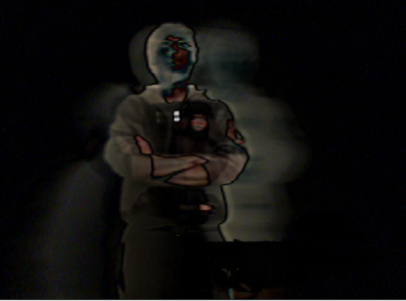
\includegraphics[scale=0.65]{grayscale/grayscale_2}
	\label{fig:grayscale_2}}
	\subfigure[After grayscale filter is applied]{
	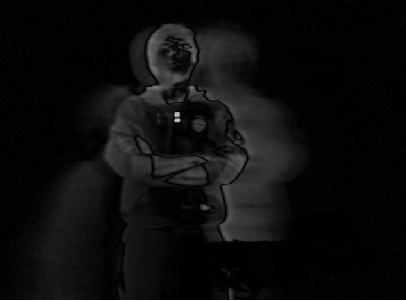
\includegraphics[scale=0.65]{grayscale/grayscale_3}
	\label{fig:grayscale_3}}
	\quad
	\subfigure[After threshold is applied]{
	
\includegraphics[scale=0.65]{threshold/threshold_1}
	\label{fig:threshold_1}}
	\subfigure[After dilation and erosion]{
	
\includegraphics[scale=0.65]{dilate_erode/dilate_erode_1}
	\label{fig:dilate_erode_1}}
	\quad
	\subfigure[After bounding box is drawn]{
	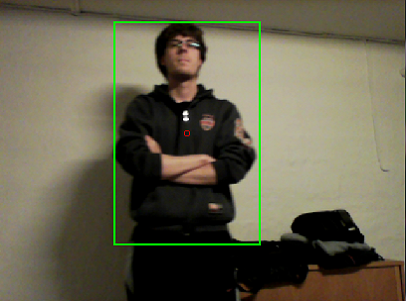
\includegraphics[scale=0.65]{bounding_box/bounding_box_1}
	\label{fig:bounding_box_1}}
	\caption{Object detection example}
	\label{fig:object_detection_example}
\end{figure}

\begin{figure}[htb]
	\centering
	\subfigure[Average time (in seconds) needed to multiply two $300 \times 300$ size matrices in Java and Python on a laptop]{
	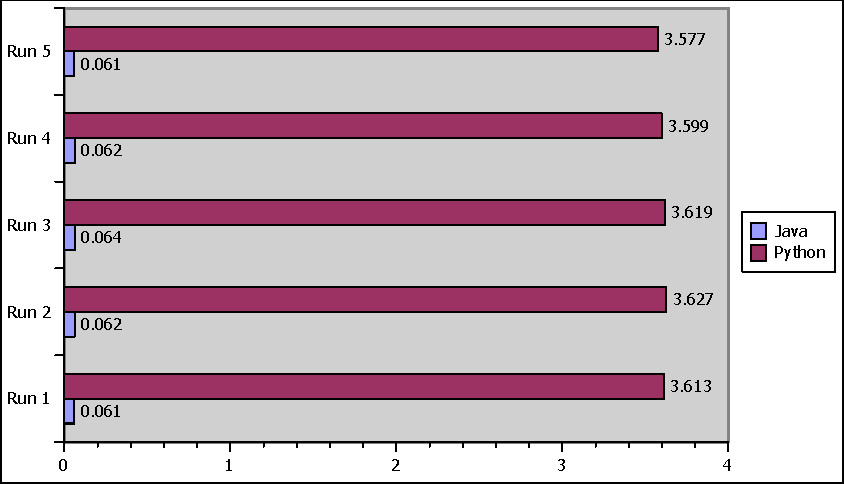
\includegraphics[scale=0.95]{benchmark/benchmark_1}
	\label{fig:benchmark_1}}
	\quad
	\subfigure[Average time (in seconds) needed to multiply two $300 \times 300$ size matrices in Java and Python on a Raspberry Pi computer]{
	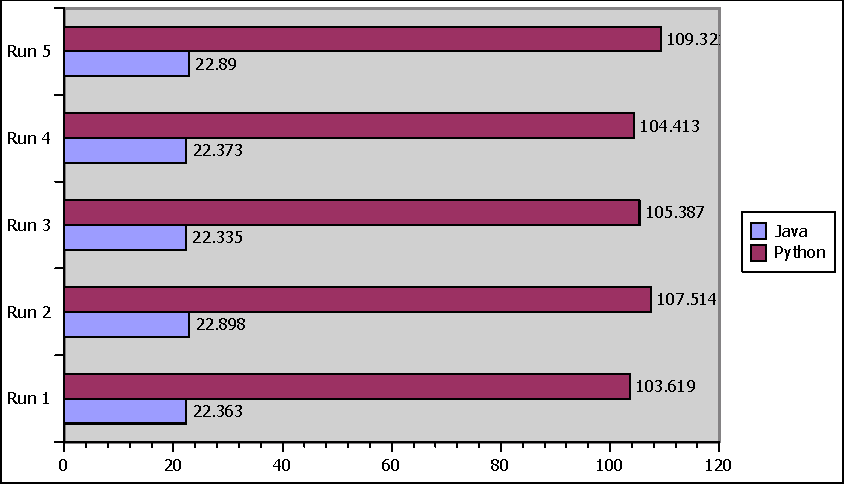
\includegraphics[scale=0.95]{benchmark/benchmark_2}
	\label{fig:benchmark_2}}
	\caption{Benchmark of matrix multiplication of two $300 \times 300$ size matrices}
	\label{fig:benchmark_multiplication}
\end{figure}

\begin{figure}[htb]
	\centering
	\subfigure[Average time (in seconds) needed to process images in Java and Python on a laptop]{
	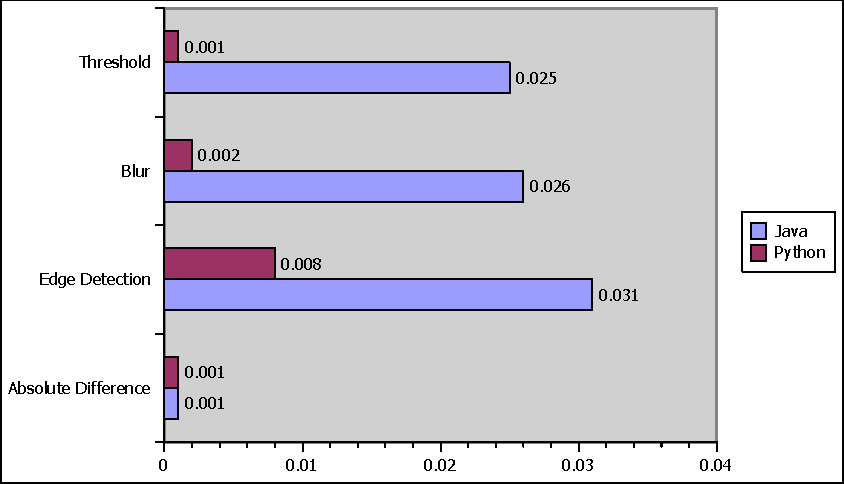
\includegraphics[scale=0.95]{benchmark/benchmark_3}
	\label{fig:benchmark_3}}
	\quad
	\subfigure[Average time (in seconds) needed to process images in Java and Python on a Raspberry Pi computer]{
	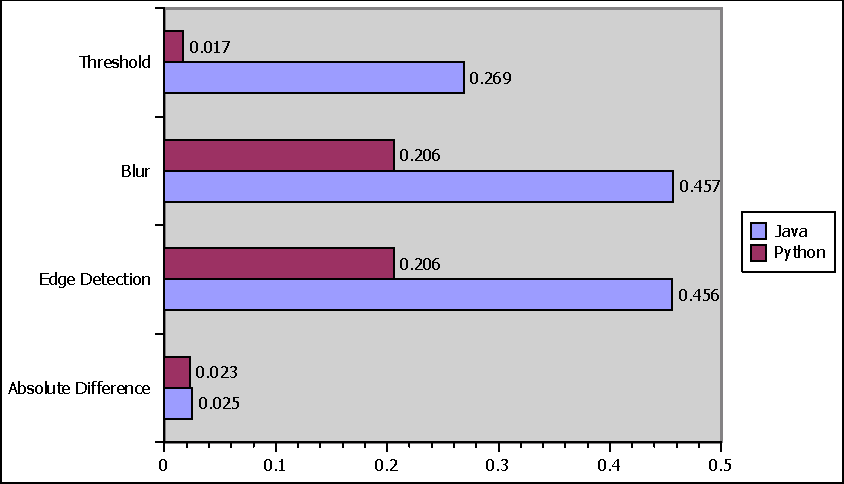
\includegraphics[scale=0.95]{benchmark/benchmark_4}
	\label{fig:benchmark_4}}
	\caption{Benchmark of image processing}
	\label{fig:benchmark_image_processing}
\end{figure}

\chapter{Appendix B}
\label{app:appendixB}
\section{Member Profiles} \label{sec:member_profiles}
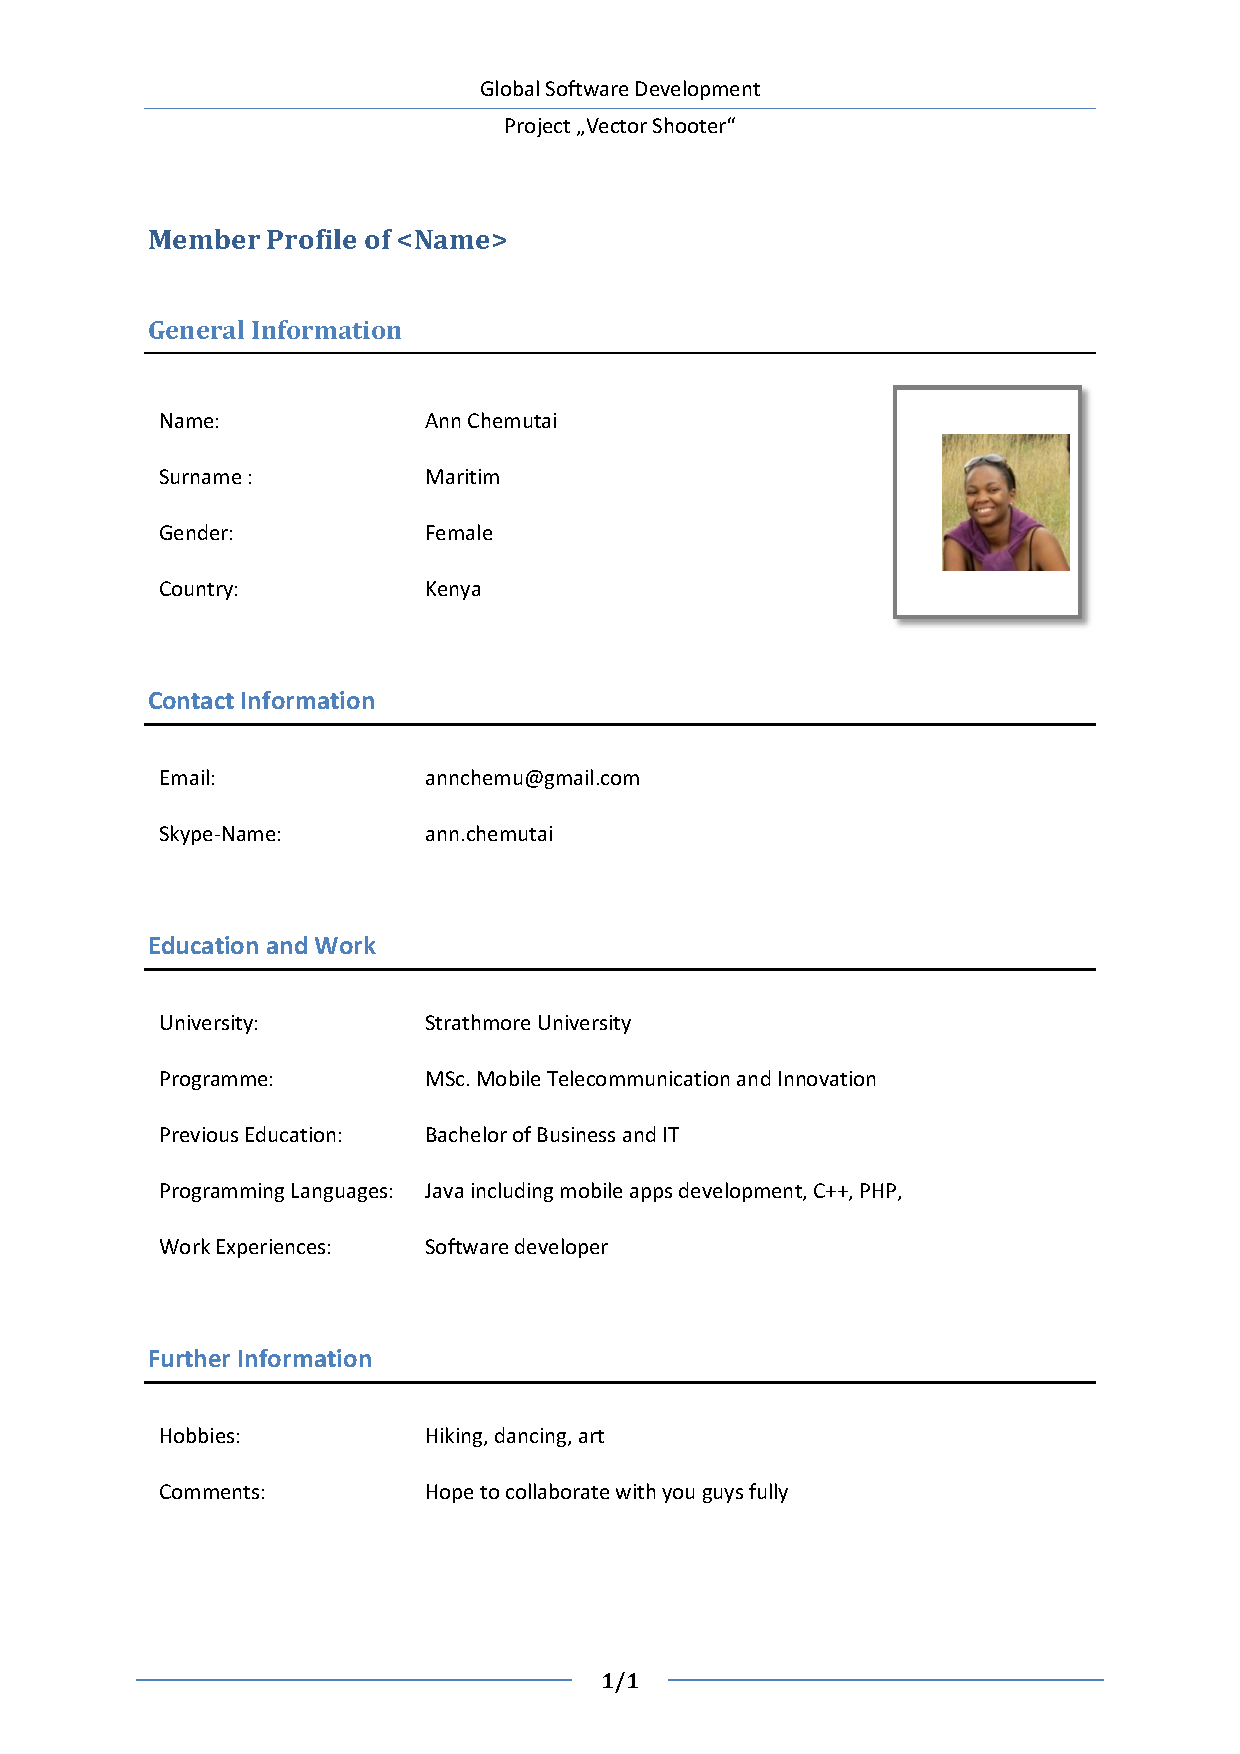
\includepdf[pages={-}]{appendix/MemberProfile_Ann.pdf}
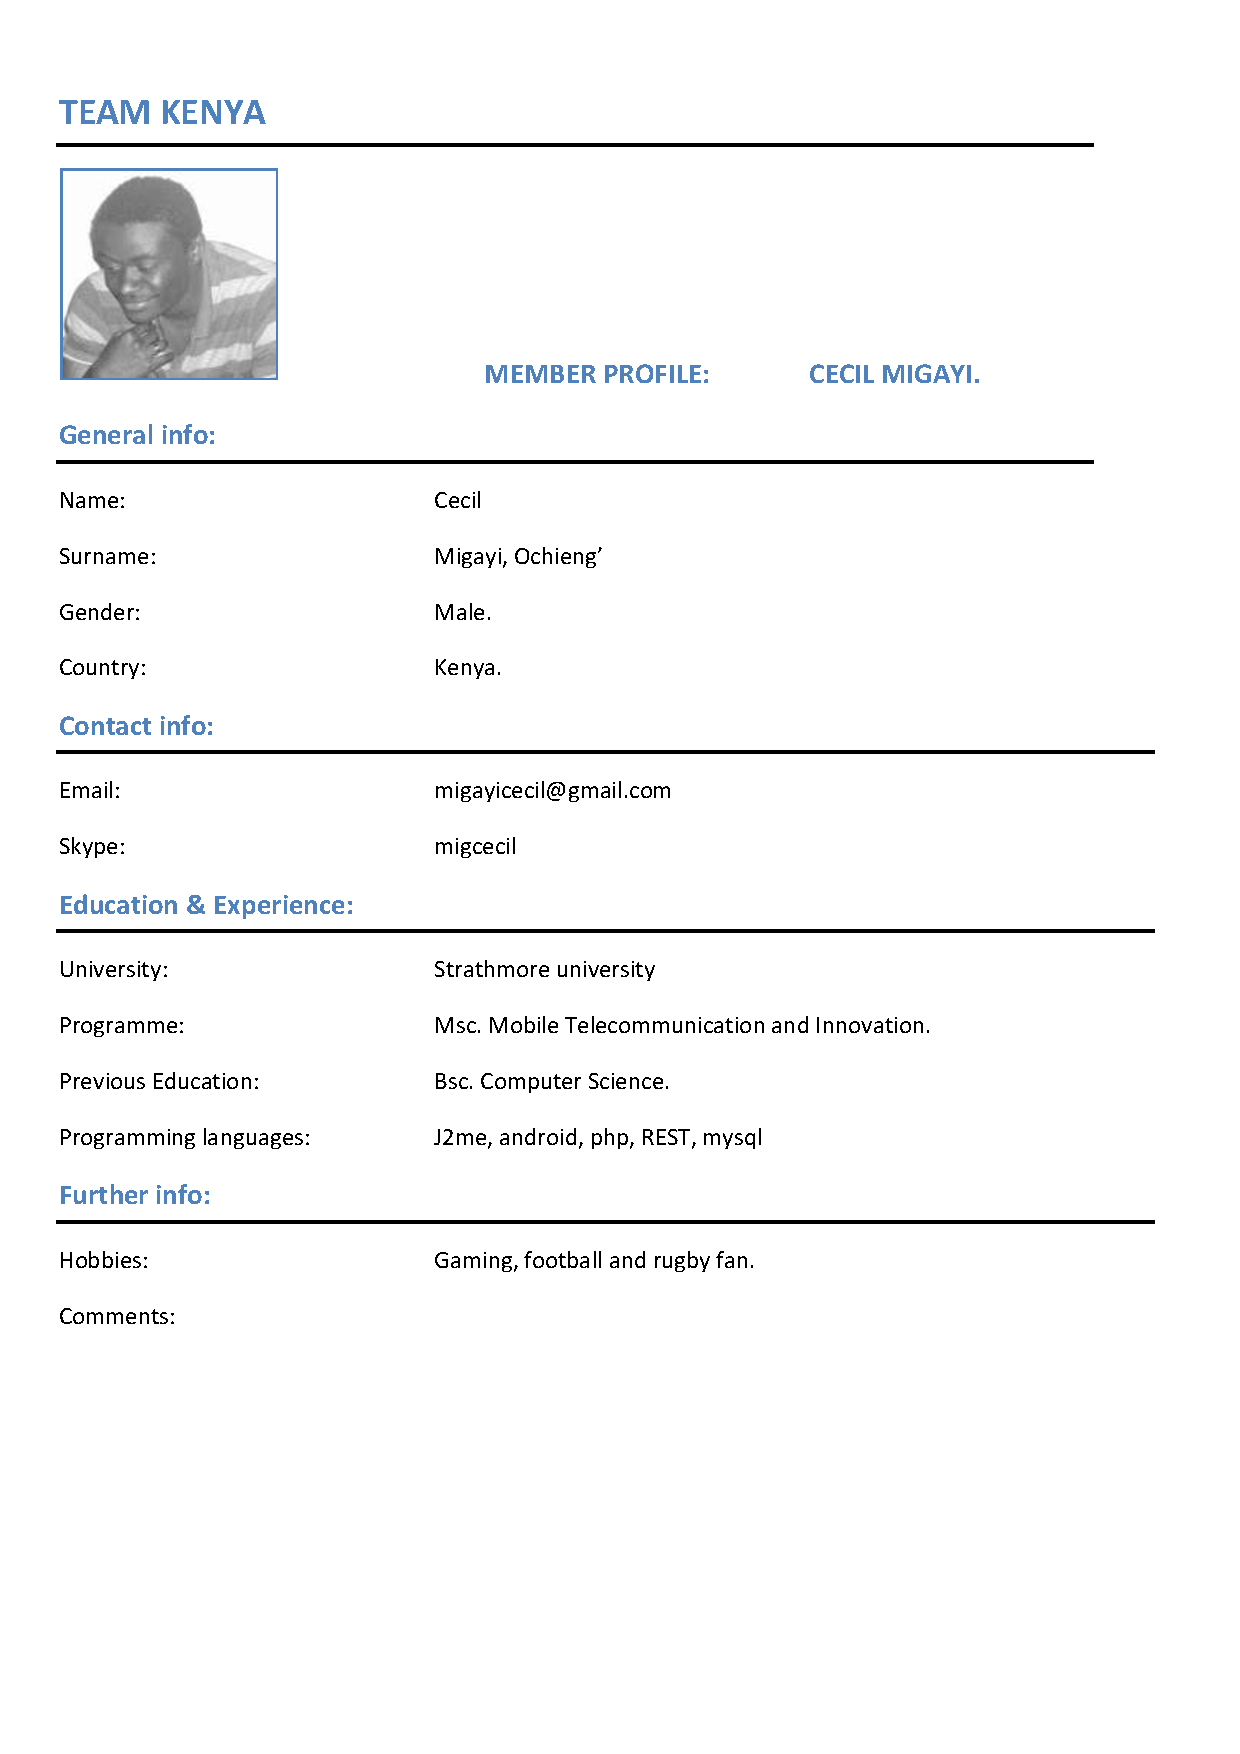
\includepdf[pages={-}]{appendix/MemberProfile_Cecil.pdf}
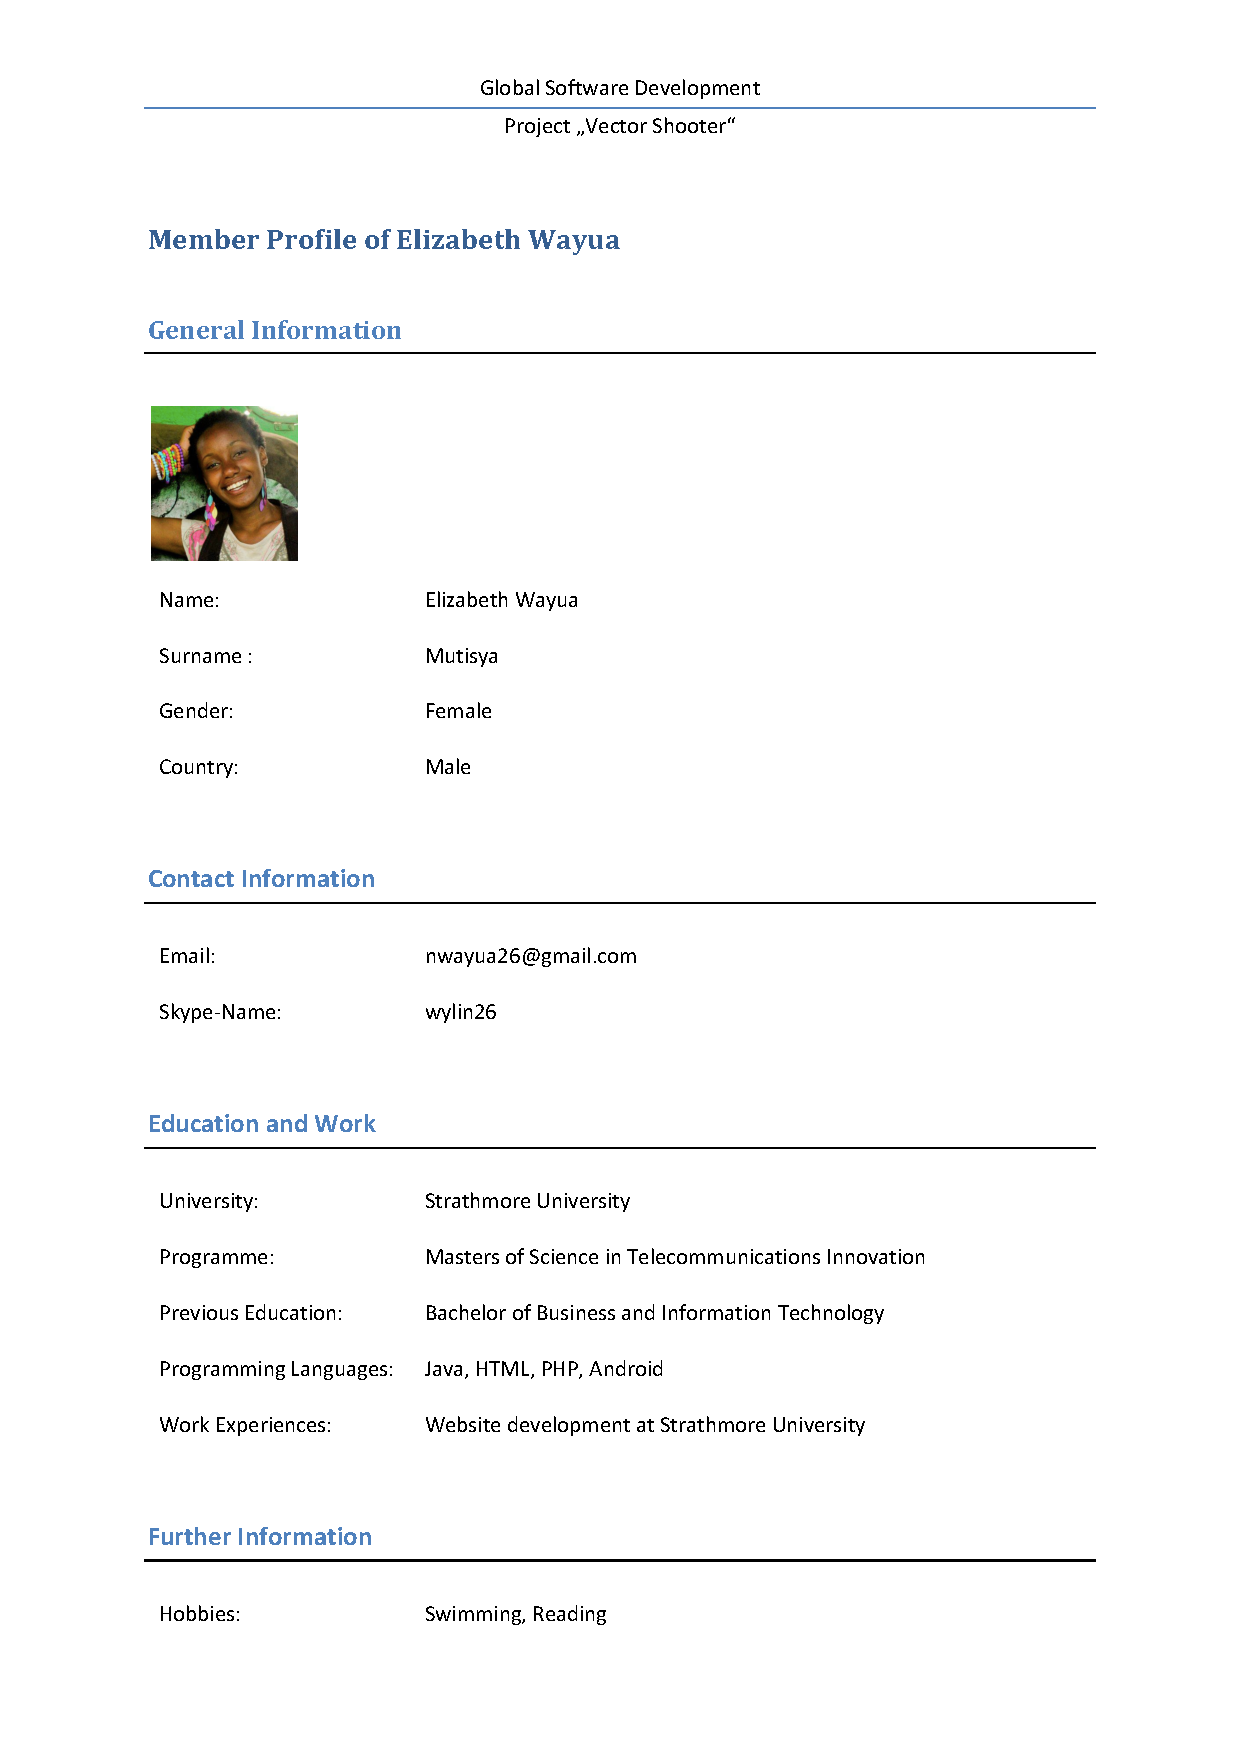
\includepdf[pages={-}]{appendix/MemberProfile_Wayua.pdf}
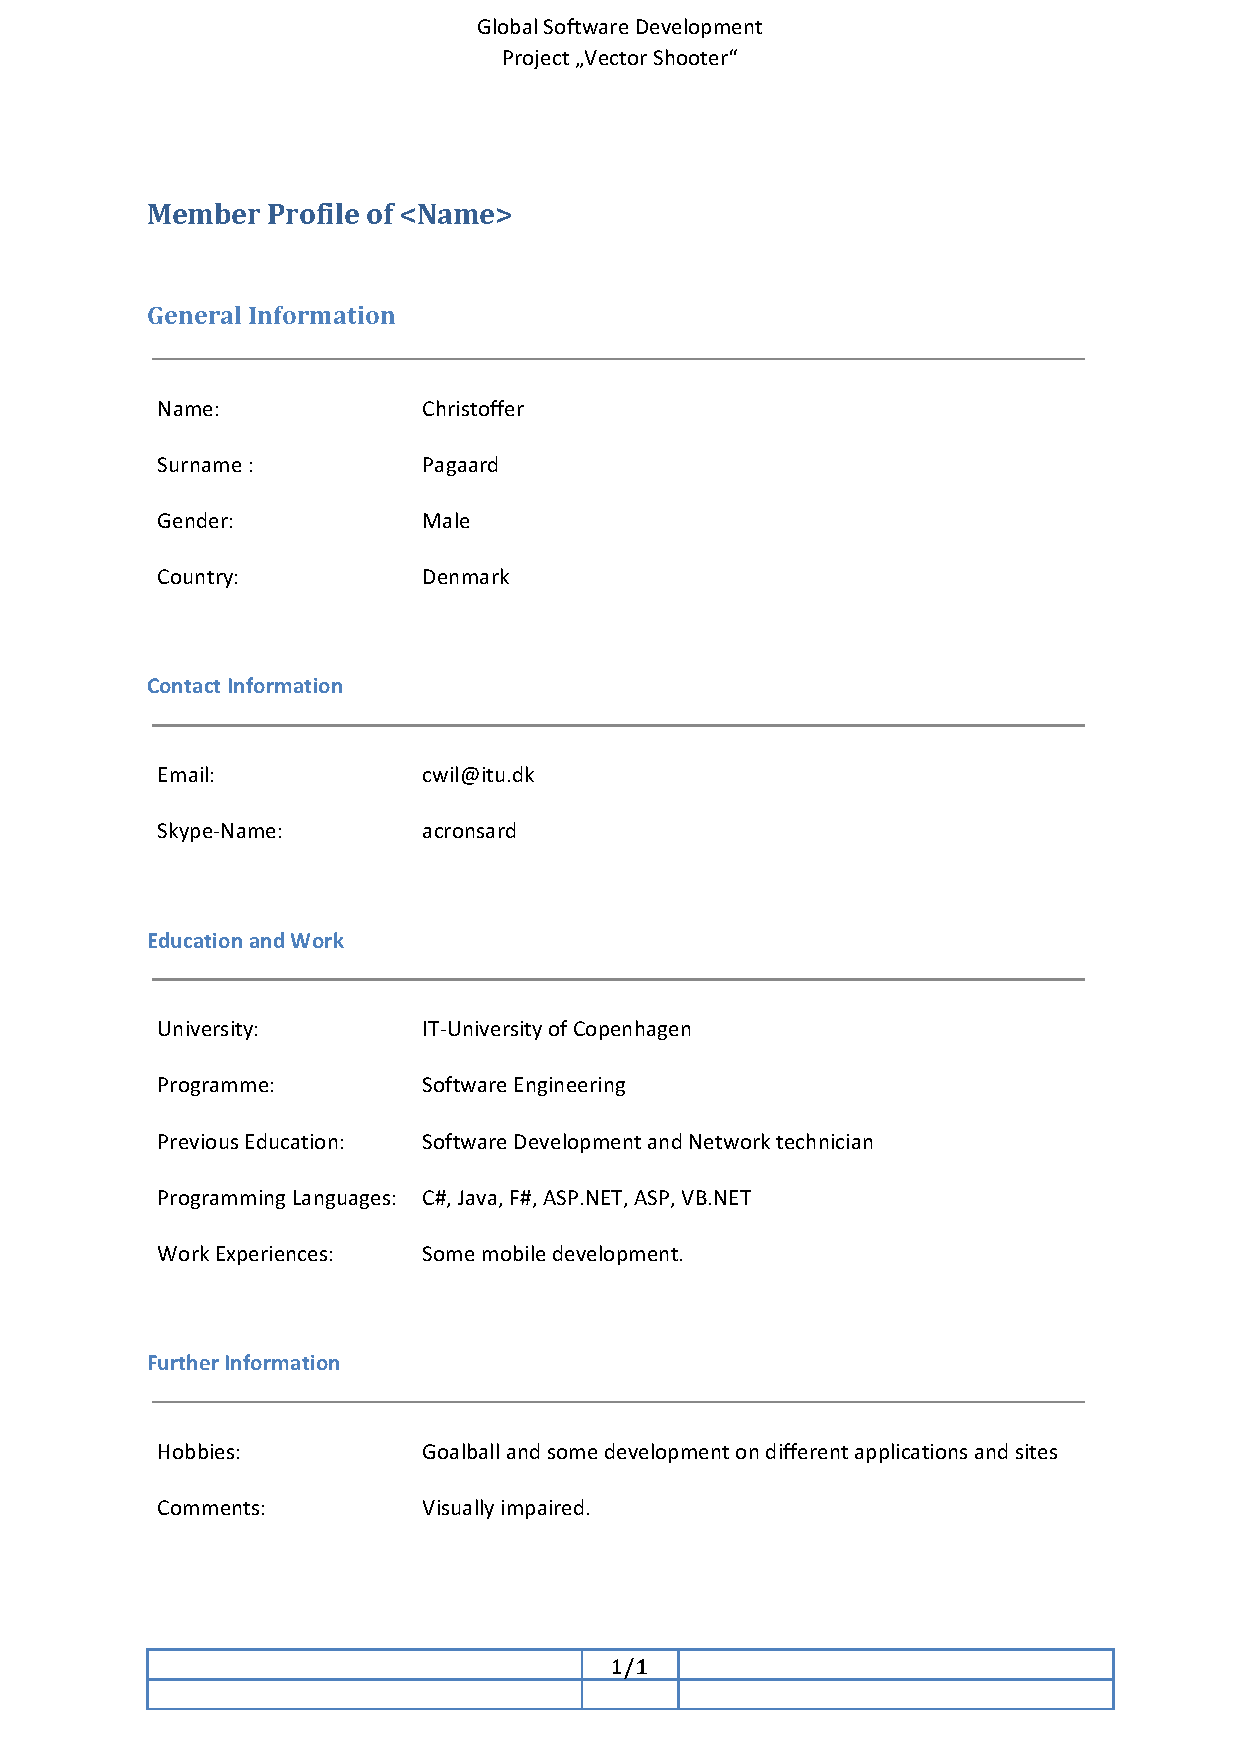
\includepdf[pages={-}]{appendix/MemberProfile_CWIL.pdf}
\includepdf[pages={-}]{appendix/MemberProfile_JRRA.pdf}
\includepdf[pages={-}]{appendix/MemberProfile_TEBR.pdf}
\includepdf[pages={-}]{appendix/MemberProfile_TMIS.pdf}

\section{Skill-/Preference-Sheet} \label{sec:Skill_Preference_Sheet}
\includegraphics[scale=0.75,angle=90]{appendix/Skill_Preference_Sheet.pdf}

\section{Motivation-Sheet} \label{sec:Motivation_Sheet}
\includegraphics[scale=0.95,angle=90]{appendix/Motivation_Sheet.pdf}

\section{"Out-of-Office"-Calendar} \label{sec:Calendar}
\includegraphics[scale=0.7,angle=90]{appendix/Calendar.pdf}

\section{Global Meeting Reports}
\includepdf[pages={-},link,linkname=GSD20131001]{appendix/GlobalMeetingReport_20131001.pdf}
\includepdf[pages={-},link,linkname=GSD20131024]{appendix/GlobalMeetingReport_20131024.pdf}
\includepdf[pages={-},link,linkname=GSD20131031]{appendix/GlobalMeetingReport_20131031.pdf}
\includepdf[pages={-},link,linkname=GSD20131112]{appendix/GlobalMeetingReport_20131112.pdf}
\includepdf[pages={-},link,linkname=GSD20131119]{appendix/GlobalMeetingReport_20131119.pdf}
\includepdf[pages={-},link,linkname=GSD20131126]{appendix/GlobalMeetingReport_20131126.pdf}
\includepdf[pages={-},link,linkname=GSD20131203]{appendix/GlobalMeetingReport_20131203.pdf}

\section{Emails}

\section{Survey}

\listoftodos
\todo{Some note or other.}
\todo[noline]{Another note.}
\todo[inline]{And another one.}
\missingfigure{Add my picture here.}

\end{document}